\documentclass[preprint,12pt]{elsarticle}

\usepackage{lineno,hyperref}
\modulolinenumbers[5]

\usepackage{booktabs} % For formal tables
\usepackage{hyperref}       % hyperlinks
\usepackage{url}            % simple URL typesetting
\usepackage{booktabs}       % professional-quality tables
\usepackage{amsfonts}       % blackboard math symbols
\usepackage{nicefrac}       % compact symbols for 1/2, etc.
\usepackage{microtype}      % microtypography
\usepackage{cleveref}
\usepackage{amsmath,amssymb,amsthm}             % AMS Math
\usepackage{dsfont}
\usepackage{mathtools}
\usepackage{amsthm}

\usepackage{algorithm}
\usepackage{algpseudocode}

\usepackage{tikz}

\usepackage{array}
\usepackage{multirow}

\usetikzlibrary{shapes,backgrounds, calc, shadings, arrows,decorations.pathmorphing,backgrounds,fit,positioning,shapes.symbols,chains}
\pgfdeclareradialshading{ballshading}{
 \pgfpoint{-10bp}{10bp}}
 {color(0bp)=(gray!50!black);
  color(9bp)=(gray!50!black);
  color(18bp)=(gray!50!black);
  color(25bp)=(gray!50!black);
  color(50bp)=(black)}

\tikzstyle{peers}=[draw,circle, minimum width=10pt]
\tikzstyle{superpeers}=[draw,circle,minimum width=20pt]

\tikzset{
%Define standard arrow tip
>=stealth',
%Define style for different line styles
help lines/.style={dashed, thick},
axis/.style={<->},
important line/.style={thick},
connection/.style={thick, dotted},
}
\newcommand\A{\ensuremath{\mathcal{A}}}
\newcommand\B{\ensuremath{\mathcal{B}}}

\newcommand\cmbox[1]{
  \fbox{\lower0.75cm
    \vbox to 1.0cm{\vfil
      \hbox to 1.7cm{\hfil\parbox{1.4cm}{\centering #1}\hfil}
      \vfil}%
  }%
}

\newcommand\cmlegend[1]{
  {\lower0.75cm
    \vbox to 1.0cm{\vfil
      \hbox to 0.7cm{\hfil #1}
      \vfil}%
  }%
}


\newtheorem{assumption}{Assumption}



\DeclareMathOperator*{\arginf}{arg\,inf}
\DeclareMathOperator*{\argmin}{arg\,min}
\DeclareMathOperator*{\argmax}{arg\,max}


\def\HCBR{{\sc HCBR}}
\def\bfHCBR{{\sc \bf HCBR}}

\newcommand{\mynote}[1]{{\bf  \textcolor{blue}{#1}}}


\theoremstyle{definition}
\newtheorem{definition}{Definition}[section]

\journal{Information Systems}

%%%%%%%%%%%%%%%%%%%%%%%
%% Elsevier bibliography styles
%%%%%%%%%%%%%%%%%%%%%%%
%% To change the style, put a % in front of the second line of the current style and
%% remove the % from the second line of the style you would like to use.
%%%%%%%%%%%%%%%%%%%%%%%

%% Numbered
%\bibliographystyle{model1-num-names}

%% Numbered without titles
%\bibliographystyle{model1a-num-names}

%% Harvard
%\bibliographystyle{model2-names.bst}\biboptions{authoryear}

%% Vancouver numbered
%\usepackage{numcompress}\bibliographystyle{model3-num-names}

%% Vancouver name/year
%\usepackage{numcompress}\bibliographystyle{model4-names}\biboptions{authoryear}

%% APA style
%\bibliographystyle{model5-names}\biboptions{authoryear}

%% AMA style
%\usepackage{numcompress}\bibliographystyle{model6-num-names}

%% `Elsevier LaTeX' style
\bibliographystyle{elsarticle-num}
%%%%%%%%%%%%%%%%%%%%%%%

\begin{document}

\begin{frontmatter}

\title{Binary Classification in Unstructured Space With Hypergraph Case-Based Reasoning}

%% Group authors per affiliation:
\author{Alexandre Quemy}
\address{IBM Krakow Software Lab, Cracow, Poland}
\ead{aquemy@pl.ibm.com}
\address{Faculty of Computing, Pozna\'n University of Technology, Pozna\'n, Poland}


\begin{abstract}
Binary classification is one of the most common problem in machine learning. It consists in predicting whether a given element is of a particular class. In this paper, a new algorithm for binary classification is proposed using a hypergraph representation. Each element to be classified is partitioned according to its interactions with the training set. For each class, the total support is calculated as a convex combination of the {\it evidence} strength of the element of the partition. The evidence measure is pre-computed using the hypergraph induced by the training set and iteratively adjusted through a training phase. It does not require structured information, each case being represented by a set of {\it agnostic information} atoms. Empirical validation demonstrates its high potential on a wide range of well-known datasets and the results are compared to the state-of-art. The time complexity is given and empirically validated. Its capacity to provide good performances without hyperparameter tuning compared to standard classification methods is studied. Finally, the limitation of the model space is discussed and some potential solutions proposed.
\end{abstract}


\begin{keyword}
binary classification, hypergraph, case-base reasoning
%\MSC[2010] 00-01\sep  99-00
\end{keyword}

\end{frontmatter}

\linenumbers


%%%%%%%%%%%%%%%%%%%%%%%%%%%%%%%%%%%%%%%%%%%%%%%%%%%%%%%%%%%%%%%%%%%%%%%%%%%%%%%
\section{Introduction}\label{sec:intro}
%%%%%%%%%%%%%%%%%%%%%%%%%%%%%%%%%%%%%%%%%%%%%%%%%%%%%%%%%%%%%%%%%%%%%%%%%%%%%%%

In many real-life situations, one tries to take a decision based on previous {\it similar} situations. Each situation is described by a certain amount of information, either collected by an expert according to the relevance of the information, or automatically by some sensors or algorithms. Those situations share similarities on which to make analogies or counter-examples in order to take a new decision. Conversely, in general, if two situations do not share any common characteristic, then they are totally independent, i.e. it is impossible to infer one's outcome from the other one. The purpose of supervised machine learning algorithms is to exploit the available information and interactions between past cases or examples in order to build a model or infer the key rules to take correct decisions.

Due to the large variety of concrete situations that can be reduced to binary classification, it is one of the most studied problems in machine learning. In this paper, we investigate the problem of binary prediction under a supervised setting, i.e. given a history of previous situations labeled with the correct output.

This paper {\bf contributes} to binary classification with a new algorithm called Hypergraph Case-Based Reasoning (\HCBR). The idea is to create a hypergraph where each element of the training set is a hyperedge and vertices are represented by the features describing the elements. The intersections between edges create a partition unique to a hypergraph. For each case, we model the support as a convex combination of the elements of this partition. Each of those elements is valued according to its importance w.r.t. to the set of all the hyperedges it belongs to and their respective labels.

The paper is an extension of \cite{DBLP:conf/dolap/Quemy18} with a focus on separating the abstract framework from the specific implementation used for the experiments. On top of the previous comparison to the best literature results, we extended the empirical validation with a comparison between \HCBR~ and 9 alternative methods for binary classification, showing the robustness of our approach. A study of learning curves and model spaces, highlighted some properties of \HCBR~ and the limitation of the current model space, thus shaping priority axes for future work. Among other refinements, we provided matricial formulation for the model space and model selection to ease an efficient implementation. We also showed more evidence concerning the model calibration.

The well-known ``no free lunch'' theorem states that there is no unique algorithm that can outperform all the others in supervised learning. The advantages of a an algorithm on a particular domain, problem or even instance is ``paid'' on another. However, the case description and representation play a preponderant role in the performances. Yet the algorithms are very often constrained by being designed to a specific representation that may not be suitable for a given problem or user data. The proposed method is totally agnostic about the data representation\footnote{With the exception that the current version must work with discrete representation.} and does not require the data to be structured. For instancewrongly, it can work on atomic representations such as Bag-of-Word representations for texts where an atom is a single word (or $n$-gram). In this case, two elements would not have the same number of elements and it may be hard to properly define the feature domain.

The plan of the paper is as follows: in Section \ref{sec:problem} the problem of binary classification is formalized and a more general formulation in an abstract space of information is proposed. We illustrate the interest of such formulation by practical constraints. The main contribution of this paper is divided into two parts: Section \ref{sec:hcbr} defines the general \HCBR~ framework and its particular instance we used in practice. Section \ref{sec:experiments} presents empirical results on seven datasets from the UC Irvine Machine Learning Repository (UCI)\footnote{\href{http://archive.ics.uci.edu/ml/index.php}{http://archive.ics.uci.edu/ml/index.php}} and the LIBSVM\footnote{\href{https://www.csie.ntu.edu.tw/~cjlin/libsvmtools/datasets/binary.html}{https://www.csie.ntu.edu.tw/~cjlin/libsvmtools/datasets/binary.html}}. The paper ends in Section \ref{sec:conclusion} with a discussion about the results, future work, and possible improvements.


\section{Binary Classification}
\label{sec:problem}

Before introducing the problem of binary classification, we present the notations used throughout this paper. Vectors are denoted in bold and small case (e.g. $\mathbf x$) and their component in small case (e.g. $x_i$). A collection of vectors is denoted in bold and large case (e.g. $\mathbf X$). $|\mathbf x|$ (resp. $|\mathbf X|$) denotes the cardinal of the vector $\mathbf x$ (resp. the collection $\mathbf X$) while $||\mathbf x||$ is its norm. The scalar product is denoted by $<.,.>$. For a matrice $A = (a_{ij})$, $a_{i:}$ is the $i$th row vector and $a_{:j}$ the $j$th column vector. 

In machine learning, the problem of classification consists in finding a mapping from an input vector space $\mathcal X$ to a discrete decision space $\mathcal Y$ using a set of examples. The binary classification problem is a special case such that $\mathcal Y$ has only two elements. It is often viewed as an approximation problem s.t. we want to find an estimator $\bar J$ of an unknown mapping $J$ available only through a sample called {\it training set}. A training set $(\mathbf{X}, \mathbf{y})$ consists of $N$ input vectors $\mathbf{X} = \{ \mathbf{x}_1, ..., \mathbf{x}_N \}$ and their associated correct class $\mathbf{y} = \{ J(\mathbf{x}_i) \}^{N}_{i=1}$.

Let $\mathcal{J}(\mathcal X, \mathcal Y)$ be the class of mappings from $\mathcal X$ to $\{-1,1\}$, or simply $\mathcal{J}$ if there is no ambiguity. A machine learning algorithm to solve binary classification is an application $\mathcal A: \mathcal{X}^N \times \mathcal{Y}^N \mapsto \mathcal{J}$ capable of providing a good approximation for any $J \in \mathcal{J}$ under some assumptions on the {\it quality} of the training set. In practice, it is not reasonable to search directly in $\mathcal{J}$ and some assumptions on the ``shape'' of $J$ are made s.t. $\bar J = \mathcal{A}(\mathbf{X}, \mathbf{y})$ belongs to a {\it hypothesis} space or model space $\mathcal H \subset \mathcal{J}$. This restriction implies not only that the exact mapping $J$ is not always reachable but might also not be approximated correctly by any element of $\mathcal H$. The choice of the model space is thus crucial as it should be large enough to represent fairly complex functions and small enough to easily find the best approximation of a given mapping $J$.

In general, a robust classification algorithm must able to approximate correctly any possible mapping. The problem of finding such algorithm consists in minimizing the generalization error for all possible mappings. Formally, it consists in solving:
\begin{equation}
\label{eq:pb}
\underset{\mathcal A}{\min} \sum_{J \in \mathcal{J}} \int_{\mathcal{X}} ||J(\mathbf{x}) - \bar J(\mathbf{x}) ||\mu(\mathbf{x}) \mathop{dx}
\end{equation}.

In practice, the generalization error cannot be computed and the set of possible mappings is unreasonably large. For those reasons, we aim at minimizing the empirical classification error on a reasonably large set of datasets $\mathcal D =  \{ (\mathbf{X}_1, \mathbf{y}_1), ..., (\mathbf{X}_K, \mathbf{y}_K)  \}$, i.e.
\begin{equation}
\underset{\mathcal A}{\min} \sum_{(\mathbf{X}, \mathbf{y}) \in \mathcal D}  \sum_{ (\mathbf{x}, y) \in (\mathbf{X}, \mathbf{y})} \mathbb{I}_{\{y \neq \bar J(\mathbf{x})\}}
\end{equation}.

To highlight the differences between standard classification problem and our approach, we briefly present linear models for classification followed by the classification in unstructured space. We also present classification on hypergraphs to discuss how the standard approach is not suitable for our purposes.

\subsection{Linear Binary Classification}


The problem of binary classification is commonly studied with $\mathcal{X} = \mathbb{R}^{M}$. Many popular classification approaches such as SVM, perceptron or logistic regression define the model space as the set of $M$-hyperplan. A $M$-hyperplan is uniquely defined by a vector $\mathbf{w} \in \mathbb{R}^{M}$ and a bias $w_0 \in \mathbb{R}$ and can be explicited by
\begin{align}
 \label{eqn:hyperplan}
 h_{\mathbf{w}}(\mathbf{x}) = <{\mathbf{w}}, {\mathbf{x}}> + w_0 = 0
\end{align} The {\it homogeneous} notation consists in adding $w_0$ to $\mathbf{w}$ by rewritting $\mathbf{x}$ such that $\mathbf{x} = (1, x_1, ..., x_M)$. The hyperplan equation \eqref{eqn:hyperplan} is then expressed by $h_{\mathbf{w}}(\mathbf{x}) = <{\mathbf{w}}, {\mathbf{x}}>$.
A hyperplan separates $\mathbb{R}^{M}$ into two regions, and thus, can be used as a discriminative rule such that 
\begin{align}
 \bar J_{\mathbf{w}}(x) = \left\{\begin{matrix}
1 & ~h_{\mathbf{w}}(\mathbf{x}) > 0\\ 
-1 & ~h_{\mathbf{w}}(\mathbf{x}) \leq 0
\end{matrix}\right.
\end{align}
Then,  given a training set $(\mathbf{X}, \mathbf{y})$, the classification problem is equivalent to find the best hyperplan such that it minimizes a certain {\it loss} function over the training set:
\begin{align}
 \label{eqn:param_model}
\mathbf{w}^* = \underset{\mathbf{w}}{\argmin} ~ \underset{i=1}{\overset{N}{\sum}} L(\mathbf{w}, \mathbf{x_i}) + \lambda R(\mathbf{w})
\end{align} where $R(\mathbf{w})$ is {\it regularization} term to prevent overfitting (usually $||w||^2_2$ or $||w||_1$) and $\lambda > 0$ a hyperparameter controlling the effect of regularization. Note that \eqref{eqn:param_model} is a parametric problem due to the choice of model space. Several losses functions exists, and are generally based on the {\it margin} of $\mathbf{x}_i$ which is defined by $m(\mathbf{w}, \mathbf{x_i}) = J(\mathbf{x_i}) h_{\mathbf{w}}(\mathbf{x}_i)$. The margin represents the distance of a vector $\mathbf{x_i}$ to the hyperplan defined by $h_{\mathbf{w}}$. It is positive if $\mathbf{x_i}$ is correctly classified, negative otherwise. For the most known, the 0-1 loss, hinge loss and log loss are defined by
\begin{align}
  \begin{matrix}
    L_{01}(\mathbf{w}, \mathbf{x})\hfill  = & \mathbb{I}_{\{ m(\mathbf{w}, \mathbf{x}) \leq 0 \}} \hfill \\
    L_{\text{hinge}}(\mathbf{w}, \mathbf{x})\hfill  = & \max(0, 1 - m(\mathbf{w}, \mathbf{x})) \\
    L_{\log}(\mathbf{w}, \mathbf{x})\hfill  = & \ln(1 + e^{- m(\mathbf{w}, \mathbf{x})}) \hfill
  \end{matrix}
\end{align}
The Perceptron algorithm uses the 0-1 loss, while SVM minimizes the hinge loss and the Logistic Regression the log loss.


%%%%%%%%%%%%%%%%%%%%%%%%%%%%%%%%%%%%%%%%%%%%%%%%%%%%%%%%%%%%%%%%%%%%%%%%%%%%%%%
\subsection{On the necessity of unstructured spaces}
%%%%%%%%%%%%%%%%%%%%%%%%%%%%%%%%%%%%%%%%%%%%%%%%%%%%%%%%%%%%%%%%%%%%%%%%%%%%%%%
\label{sec:bc_unstructured}

In this paper, we relax the three following implicit constraints on the input vector space:
\begin{enumerate}
\item we do not assume to have any inner product or metric embedded with the input vector space,
\item we do not assume the cardinality of the input vectors, such that it is possible to build a model and make predictions on incomplete systems (for instance missing values in some rows in a database or Bag-of-Words representation),
\item we do not assume anything about the concrete {\it representation} of features while in most classification methods, all the features belongs to the same space, often $\mathbb{R}$.
\end{enumerate}
Most of classification methods work directly in the feature space, or, when they modify it, the resulting space inherits the topology of the initial space. In the particular case of linear models, a scalar product is mandatory to represent the decision itself and to quantify the distance from an element to the decision boundary. In some cases, a metric is obviously available, and in some other cases some ad-hoc metrics may be constructed for a specific problem. However, there a plenty of practical situations where the {\it good} metric is not known (e.g. it requires a very specific expertise). Also, it is very common to miss some data in a dataset (e.g. due to a defective sensor for some period of time), or to have to include new pieces of information after an initial model was built (e.g. adding new sensors). In the case of SVM, for instance in $\mathbb{R}^3$, if an element has only 2 components it does not describe a point but a plan and as a result, there is no way separate it with a (hyper)plan. 

Conversely, consider a model built in $\mathbb{R}^2$ with some additional information available after such that the classification instance now lives in $\mathbb{R}^3$. Mathematically, there is no guarantee that the model in two dimensions is even close to the model built from scratch in three dimensions. For instance, if the points are not linearly  separable in two dimensions but are in three dimensions, there is no chance for the projection of the plane into the subspace of two dimensions to be the model found while working only in this subspace. Despite multiple algorithms have an {\it online} counterpart, i.e. the model keeps being trained with new input vectors, as far as we know, there is no significant work on having this {\it horizontal} scalability (as opposed to vertical scalability). One step toward horizontal scalability is to work only in unstructured spaces.
Last, the features representation is very often imposed by the classification method itself and when the dataset does not respect those requirements, it has to be transformed. Of course, exploiting the specificities of features often lead to better results but also requires manual expertise that blocks a wider adoption by end-users. This is particularely true with categorical variables that often require to be encoded taking into account the method specificity. For instance, for Decision Tree and its Ensemble counterpart, the Random Forest, the accuracy depends on the encoder and using a Numerical encoder, a One-Hot encoder or a Binary encoder may drastically change the model fitted on the same data. For this reason, it is also important to develop methods that are ``agnostic'' to the data representation or at least as less sensitive as possible.

\subsection{Binary Classification In Unstructured Spaces}

With all those considerations in mind, we reformulate the problem of binary classification for unstructured space. The idea is that the only {\it ad-hoc} operation we allow is checking if a particular feature belong to the element to classify, and by extension we allow elementary set operations. We consider a countable space $\mathbb{F}$ and define $\mathcal X = 2^{\mathbb{F}}$. By abuse of notation, we call   $\mathbf{x} \in \mathcal X$ an ``input vector'' despite $\mathcal X$ is not a vector space. We also refer to $\mathbf{x}$ as a {\it case}. In practice, it is very likely that only a subset of $2^{\mathbb{F}}$ may appear (for instance if two features encode two contradictory propositions or if every case has the same number of features).
The real class for any input vector $\mathbf{x}$ of $2^{\mathbb{F}}$ is given by the mapping:
\begin{align}
    \label{assumption_mapping}
   J \colon 2^{\mathbb{F}} & \to \{-1,1 \} \\
   \mathbf{x} &\mapsto J(\mathbf{x})
\end{align}
Assuming the unknown mapping takes value from the powerset of $\mathbb{F}$ allows us not to have to know $\mathbb{F}$ at all. We could propose a more general formulation, and in particular to handle continuous space, s.t. $\mathcal X$ is defined as a $\sigma$-algebra on $\mathbb F$. However, this paper focuses on the specific case where $\mathbb{F}$ is supposed countable and the $\sigma$-algebra is defined by the powerset of $\mathbb{F}$. We let the general case for future work.

Notice that in this paper we do not consider {\it uncertainty}: if two situations are described the same in $\mathbb{F}$, then they have the same label.

\subsection{Classification and Hypergraph}
\label{sec:state_of_art}

Hypergraphs generalize graphs and can be used to represent higher order relations while graphs are limited to binary relations. A hypergraph is defined by a set of vertices and a collection of hyperedges where each hyperedge is a subset of this set of vertices. Therefore, a graph is a special case of hypergraph for which each hyperedge contains only two vertices. We will formally introduce hypergraphs in Section \ref{sec:rep}.
Recently hypergraphs have been used as data representation, and some classification algorithms on hypergraph have been proposed. A vast majority of approaches models the objects to classify as the set of vertices and constructs the hyperedges as the representation of a metric. This conventional approach is known as {\it neighborhood-based} hypergraph. The metric relies on some assumptions on the data or a specific representation (e.g. Zernike moment and histogram of oriented gradient to measure the distance between images in \cite{ijcai2017-387}) and for each vertex, a hyperedge is created to represent its $k$-nearest neighbors \cite{5540012}. 

The problem of classification on hypergraph consists in labeling some unlabeled vertices given a training set such that all vertices in a same hyperedge have the same label. As all the vertices are known a priori, the problem is part of transductive learning. To learn the labels, the standard approach is to minimize a cost function based on a hypergraph equivalent of a graph Laplacian \cite{ijcai2017-387,NIPS2006_3128} with a structural risk:
\begin{align}
C(\mathbf{x}) = \mathbf{x}^t \Delta \mathbf{x} + \mu ||\mathbf{x} - \mathbf{y}||^2
\end{align} where $\Delta$ is the hypergraph Laplacian, $\mu >0$ a regularization factor and $||.||$ a norm. The vector $\mathbf{y}$ represents the initial labels for all vertices with $y_i = 0$ for unlabeled vertices, a negative (resp. positive) value for label -1 or 1.

On the contrary, the {\bf method proposed in this paper} models the elements to classify as the hyperedges and the vertices as the different components of those elements. As far as we know, there is no previous work that uses this modeling choice. In addition, it does not require knowing all the elements before building the model: our approach is inductive. Contrary to the literature that focuses on the method to build the hyperedges, the proposed framework has a straightforward hypergraph construction and rather focus on model selection. Even more important, as most previous work consists in building metrics based on the features representation, it obviously conflicts with our goal of agnosticity described in the previous section.



\section{Hypergraph Case-Based Reasoning} 
\label{sec:hcbr}

In this section, we introduce our main contribution with {\bf a new framework for binary classification in unstructured spaces} called Hypergraph Case-Based Reasoning (\HCBR). The presentation is broken down into five steps. First, we present how to represent our training set as a hypergraph and how to project any element of $2^{\mathbb F}$ onto it. In a second part, we formally introduce the model space, the model parameters and the decision rule. Section \ref{sec:model_selection} is dedicated to the parameter estimation while Section \ref{sec:decision_training} focuses on the training and decision rule refinement. Before presenting experimental results, Section \ref{sec:complexity} provides the time complexity of the three main phases of the algorithm. 

\subsection{Representation And Projection}
\label{sec:rep}

Before defining the projection operator used by \HCBR~ to make prediction, we recall the definitions of a hypergraph and induced hypergraph as found in \cite{berge1984hypergraphs}. For additional results on hypergraphs, we refer the reader to this reference.

\begin{definition}[Hypergraph]
A hypergraph is defined by $H = (V, \mathbf{X})$ with $V$ a set of vertices, $\mathbf{X}$ the hyperedges such that $\forall \mathbf{x} \in \mathbf{X}, ~ \mathbf{x} \subseteq V$.
\end{definition}
\noindent
A hypergraph can be viewed as a collection of subsets $\mathbf{X}$ of a given set of vertices $V$. It is sometimes convenient to define a hypergraph solely by a collection of sets. In this case, the set of vertices, denoted $V_\mathbf{X}$, is implicitly defined as the union of edges.

\begin{definition}[Induced Subhypergraph]
The subhypergraph $H[A]$ induced by $A \subseteq V$ is defined by $H[A] = (A, \mathbf{X_A})$ with $\mathbf{X_A} = \{ \mathbf{x} \cap A ~ | ~ \mathbf{x} \cap A \neq \emptyset\}$.
\end{definition}
\begin{figure}[!h]
  \centering
  \def\firstcircle{(0,0) ellipse (1.5cm and 1cm)}
  \def\secondcircle{(80:-1cm) ellipse (1.5cm and 1cm)}
  \def\thirdcircle{(0:2cm) ellipse (1.5cm and 1cm)}
  \begin{tikzpicture}[scale=0.8, every node/.style={scale=1}]
      \begin{scope}[fill opacity=0.3]
          \filldraw[fill=gray, xscale=1.4, yscale=1.4] (-0.0,-0.0) plot [smooth cycle,tension=0.7, shift={(-4,-3.2)}] coordinates {(3,1) (5,1.2) (7,1) (8,3) (7,4.5) (5,4.5) (2,4) (1.7,2.5)};
          %\filldraw[fill=gray] (-3.5,-3.5) rectangle (4,2);
          \fill[red, rotate=30, xscale=1.4, yscale=1.4] \firstcircle;
          \fill[green, rotate=35, xscale=1.4, yscale=1.4] \secondcircle;
          \fill[blue, xscale=1.4, yscale=1.4] \thirdcircle;
          \draw[rotate=30, xscale=1.4, yscale=1.4] \firstcircle;
          \draw[rotate=35, xscale=1.4, yscale=1.4] \secondcircle;
          \draw[xscale=1.4, yscale=1.4] \thirdcircle;

      \end{scope}
      \node at (4,-2.7) {$\mathbb{F}$};
      \node at (0.5,1) {$x_1$};
      \node at (0,-2.3) {$x_2$};
      \node at (3,1) {$x_3$};

      \node at (-0.8  ,0.5) {$e_1$};
      \node at (1.4  ,0.7) {$e_2$};
      \node at (1.2  ,-0.3) {$e_3$};
      \node at (3.6  , -0.1) {$e_4$};
      \node at (2  , -0.7) {$e_5$};
      \node at (-0.4  ,-1) {$e_6$};
      \node at (1  ,-1.7) {$e_7$};
  \end{tikzpicture}
  \caption{\label{case_base} The family $\mathcal E = \{ \mathbf e_i \}_{i}$ forms the partition obtained by the union of the projection of cases and represents how the three cases share information.}
\end{figure}

A set of examples $\mathbf{X}$ can be seen as a hypergraph $H = (\mathbb F, \mathbf{X})$, i.e. such that each example is a hyperedge (Figure \ref{case_base}). In practice, we do not need to know $\mathbb{F}$ as we can always use the implicit hypergraph $H = (\mathbb{F}_{\mathbf X}, \mathbf{X})$ where $\mathbb{F}_\mathbf{X}$ is the restriction of $\mathbb{F}$ to the features that appear in the sample $\mathbf{X}$.
For any hypergraph $H = (\mathbb{F}_{\mathbf X}, \mathbf{X})$, there exists a unique partition $\mathcal{E}_H = \{\mathbf{e_i}\}^M_{i=1}$ defined by the the intersections of its edges as illustrated by Figure \ref{case_base}.

The idea of the projection of a case $\mathbf x$ over an hypergraph is to return the partition of $\mathbf x$ defined by the intersections with $\mathcal{E}_H$. In particular, the projection of a hyperedge is included in $\mathcal{E}_H$.
\begin{definition}[Projection defined by a hypergraph]
The projection operator $\pi_H$ over a hypergraph $H = (V, \mathbf{X})$ for any $A \subseteq V$ is defined by $\pi_H(A) = \{ \mathbf{e} \subseteq A ~ | ~ \exists \mathbf{X'} \subseteq \mathbf{X_A}, ~ \mathbf{e} = \underset{\mathbf{x} \in \mathbf{X'}}{\bigcap} \mathbf{x} \}$.
\end{definition}

\noindent
{\bf Example:} Each element of $\pi_H(\mathbf{x})$ is a (sub)set of features. For instance, in Figure \ref{case_base}, $\pi_H(\mathbf{x_1}) = \{ \mathbf{e_1}, \mathbf{e_2}, \mathbf{e_3}, \mathbf{e_6} \}$ and in Figure \ref{new_case_schema}, the projection of $\mathbf{x}$ (in yellow) on $H$ is represented by the family $\{ \mathbf{e'}_i \}_i$. \\

We call {\it discretionary features} of $\mathbf{x}$ (w.r.t. $H$) the (possibly empty) set of features that are not in $V_{\mathbf{X}}$, denoted $D_\mathbf{x}$. It can be interpreted as the features of $\mathbf{x}$ that do not belong to any hyperedge. If a hypergraph induced by a set of examples represents a knowledge base at a given moment, the discretionary features of $\mathbf x$ are new pieces of information that were never encountered before. \\

\noindent
{\bf Example:} Considering the hypergraph composed of $\mathbf{x_1}$ and $\mathbf{x_2}$ as illustrated by Figure \ref{case_base}, the set of discretionary features of $\mathbf{x_3}$ is $\mathbf{e_4}$. In Figure \ref{new_case_schema}, the yellow case $\mathbf{x}$ has no discretionary feature: all its features are present at least in one example.\\

\begin{figure}[!h]
  \def\firstcircle{(0,0) ellipse (1.5cm and 1cm)}
  \def\secondcircle{(80:-1cm) ellipse (1.5cm and 1cm)}
  \def\thirdcircle{(0:2cm) ellipse (1.5cm and 1cm)}
  \begin{tikzpicture}[scale=0.7, every node/.style={scale=0.7}]
      \begin{scope}[fill opacity=0.3]
          \filldraw[fill=gray, xscale=1.4, yscale=1.4] (-3.5,-3.5) plot [smooth cycle,tension=0.7, shift={(-4,-3.2)}] coordinates {(3,1) (5,1.2) (7,1) (8,3) (7,4.5) (5,4.5) (2,4) (1.7,2.5)};
          %\filldraw[fill=gray] (-3.5,-3.5) rectangle (4,2);
          \fill[red, rotate=30, xscale=1.4, yscale=1.4] \firstcircle;
          \fill[green, rotate=35, xscale=1.4, yscale=1.4] \secondcircle;
          \fill[blue, xscale=1.4, yscale=1.4] \thirdcircle;
          \draw[rotate=30, xscale=1.4, yscale=1.4] \firstcircle;
          \draw[rotate=35, xscale=1.4, yscale=1.4] \secondcircle;
          \draw[xscale=1.4, yscale=1.4] \thirdcircle;

          \fill[yellow, rotate=110, xscale=1, yscale=1, xshift=-10, yshift=15] \secondcircle;
          \draw[rotate=110, xscale=1, yscale=1, xshift=-10, yshift=15] \secondcircle;

      \end{scope}
      \node at (4,-2.7) {$\mathbb{F}$};
      \node at (0.5,1.3) {$x_1$};
      \node at (0,-2.3) {$x_2$};
      \node at (3,1) {$x_3$};

      \node at (-0.8  ,0.5) {$e_1$};
      \node at (0.2  ,0.6) {$e_1'$};
      \node at (1.5  ,0.7) {$e_2$};
      \node at (1.05  ,0.5) {$e_2'$};
      \node at (1.2  ,-0.2) {$e_3'$};
      \node at (1.675  , 0.15) {$e_3$};
      \node at (3.6  , -0.1) {$e_4$};
      \node at (2  , -0.7) {$e_5$};
      \node at (1.5 , -0.8) {$e_5'$};
      \node at (-0.6  ,-1.2) {$e_6$};
      \node at (0.3  ,-0.7) {$e_6'$};
      \node at (1  ,-1.4) {$e_7'$};
      \node at (0.5  ,-2) {$e_7$};
  \end{tikzpicture}
  \hfill
  \begin{tikzpicture}[auto, thick, scale=0.8, every node/.style={scale=0.8}, baseline={(2,-4.5)}]
    % Place super peers and connect them
    \node[superpeers, fill=red!30] (c1) at  (0,-4) {$x_1$};
    \node[superpeers, fill=blue!30] (c2) at  (2,-4) {$x_2$};
    \node[superpeers, fill=green!30] (c3) at  (-2,-4) {$x_3$};
    \node[superpeers, fill=yellow!30] (c4) at (0,0) {$x$};
    %\foreach \source/\dest in {a/b, a/c, a/d, b/c, c/d,a/e,d/e}
    %  \path (\source) edge (\dest);
     \node[peers, fill=black!10, label=above:{$e_2'$}] (e2) at (-2.5,-2) {};
     \node[peers, fill=black!10, label={[xshift=0.05cm, yshift=-0.05cm]{$e_3'$}}] (e3) at (-1.5,-2) {};
     \node[peers, fill=black!10, label={[xshift=-0.1cm, yshift=-0.05cm]{$e_5'$}}] (e5) at (-0.5,-2) {};
     \node[peers, fill=black!10, label={[xshift=0.1cm, yshift=-0.1cm]{$e_1'$}}] (e1) at (0.5,-2) {};
     \node[peers, fill=black!10, label={[xshift=-0.1cm, yshift=-0.1cm]{$e_6'$}}] (e6) at (1.5,-2) {};
     \node[peers, fill=black!10, label=above:{$e_7'$}] (e7) at (2.5, -2) {};


     \path[<-] (c4) edge (e1);
     \path[<-] (c4) edge (e2);
     \path[<-] (c4) edge (e3);
     \path[<-] (c4) edge (e5);
     \path[<-] (c4) edge (e6);
     \path[<-] (c4) edge (e7);

     \path[->] (c1) edge (e1);
     \path[->] (c1) edge (e2);
     \path[->] (c1) edge (e3);
     \path[->] (c1) edge (e6);

     \path[->] (c2) edge (e3);
     \path[->] (c2) edge (e5);
     \path[->] (c2) edge (e6);
     \path[->] (c2) edge (e7);

     \path[->] (c3) edge (e2);
     \path[->] (c3) edge (e3);
     \path[->] (c3) edge (e5);

  \end{tikzpicture}
  \caption{\label{new_case_schema} The projection of $\mathbf{x}$ on $H$ is represented by the family  $\{ \mathbf e'_i\}_i$. Under the projection lies a graph representation of $\mathbf x$ with the partition elements $\{ \mathbf e_i\}_i$ and their respective connections to the cases $\{\mathbf x_i\}_i$, in particular, $D_{\mathbf x} = \emptyset$.}
\end{figure}

For any set of features $\mathbf{x} \subseteq \mathbb F$, we define $d_H(\mathbf{x}) = \{ \mathbf{x}' \in X ~ | ~ \mathbf{x} \cap \mathbf{x}' \neq \emptyset \}$ the set of edges sharing some features with $\mathbf{x}$. In particular, the set $d_H$ can be split into $d_H^{(1)}$ and $d_H^{(-1)}$ depending on the label of the case and defined by $d_H^{(l)}(\mathbf{x}) = \{\mathbf{x}' \in d_H(\mathbf{x}) ~ | ~ J(\mathbf{x}') = l \}$. $|d_H(\mathbf{x})|$ corresponds to the number of cases the case $\mathbf{x}$ intersects while $|d_H^{(l)}(\mathbf{x})|$ counts the number of times the class $l$ is used among this set of intersecting cases. Note that if $\mathbf{x} \not \in \mathbf{X}$ and $|d_H(\mathbf{x})| = 0$, then $\mathbf{x} = D_\mathbf{x}$, i.e. the case $\mathbf{x}$ is in relation with no case in $\mathbf{X}$. In the hypergraph literature, $|d(\mathbf{x})|$ is called the {\it degree} of a hyperedge and its domain of definition is restricted to $\mathbf{X}$. Finally, to use matricial notation, we define the vectors $\mathbf d^{l} = (|d^{(l)}(\mathbf x_i)|)^N_i$.

From now, we consider only the specific hypergraph generated by the set of examples $\mathbf{X}$. For the sake of readability, we remove the subscript $H$.

\subsection{Model Space}
\label{sec:model}
As discussed in Section \ref{sec:bc_unstructured}, we relaxed some implicit constraints on the input vector space.
As a counterpart, \HCBR~ relies on two assumptions: (i) the correct class of an input vector is the result of its features only and (ii) if two input vectors $\mathbf{x}$ and $\mathbf{x}'$ do not share any feature, they are {\it independent} i.e. $\mathbf{x}$ cannot help to understand the correct class of $\mathbf{x}'$ and vice versa. If (i) is a very common assumption, often implicit, (ii) comes from the fact there is no metric on $\mathbb F$ to determine a distance between two elements s.t. we can rely only on intersections. As a result, \HCBR~  produces only {\it local} models because if a new input vector is independent of all examples, it is impossible to generate a prediction. On the contrary, a hyperplan model is {\it global} in a sense that it can produce a prediction for any element of $\mathbb{R}^M$.
An example of concrete situation for which such assumptions are natural is a justice trial. Cases are composed of some elements, and the correct label is the result of a reasoning that can possibly use analogies or counter-examples with a set of past cases on top of the legal texts. However, if a judge or lawyer wants to use $\mathbf{x}$ to justify the outcome of $\mathbf{x}'$, $\mathbf{x}'$ must have similarities with $\mathbf{x}$. 

This leads to define a model space such that the support toward one class for a given case $\mathbf x$ is only function of its projection on the hypergraph. First, we give the {\bf intuition} behind our model space. For each element $\mathbf e_i$ in the projection, we value 1) its importance in the case $\mathbf x$ and 2) its support toward a specific class given the whole hypergraph. Intuitively, 1) consists in answering the question: {\it how important is $\mathbf e_i$ w.r.t. $\mathbf x$?} or {\it what is the potential for analogies or counter-examples between $\mathbf x$ and the other examples also containing $\mathbf e_i$?} The purpose of 2) is to value how important is $\mathbf e_i$ with regards to the other elements of $\mathcal E$. For instance, to explain the case $\mathbf x$ in Figure \ref{case_base}, we will use only the elements of the projection $\pi_H(\mathbf{x_1}) = \{ \mathbf{e_1}, \mathbf{e_2}, \mathbf{e_3}, \mathbf{e_6} \}$. Without prior information, we will use the size of $\mathbf e_i$ in $\mathbf x$ to measure their importance $\mathbf x$: $\mathbf e_6'$ is the most important group of features and $\mathbf e_2'$ the least important. The way of measuring the support with regard to the whole hypergraph as well as an intuitive interpretation will be given in Section \ref{sec:model_selection}.

Let us now {\bf formally} define the model space. Given the hypergraph $H = (\mathbb F, \mathbf{X})$ defined by a training set $\mathbf{X}$ and its associated partition $\mathcal{E} = \{\mathbf{e_i}\}_i^m$ obtained using the projection defined in the previous section, the relation between an example $\mathbf{x}$ and its class is modeled by

\begin{align}
\label{eqn:model}
\left\{\begin{matrix}
s_{w, \mu}(\mathbf{x}) & = & \underset{i = 1}{\overset{M}\sum} w(\mathbf{e}_i, \mathbf{x}) \mu(\mathbf{e}_i, \mathbf{X}, \mathbf{y})% = <\mathbf{w}_i, \mathbf{\mu}_i >_{( \mathbf{X}, \mathbf{y})}
 \\
\underset{i = 1}{\overset{M}\sum} w(\mathbf{e}_i, \mathbf{x}_j) & = & 1 ~ \hfill \forall 1 \leq j \leq N \hfill\\
\underset{i = 1}{\overset{M}\sum} \mu(\mathbf{e}_i, \mathbf{X}, \mathbf{y}) & = & 1 \hfill
\end{matrix}\right.
\end{align} where $w(\mathbf{e}_i, \mathbf{x}_j) \geq 0$ model the importance of $\mathbf{e}_i$ in $\mathbf{x}_j$ and $\mu(\mathbf{e}_i, \mathbf{X}, \mathbf{y})$ the support of $\mathbf{e}_i$ for class 1 w.r.t. whole training set. For this reason, we call $\mu$ the {\it intrinsic strength} of $\mathbf e_i$. The assumption (ii) implies that if $\mathbf{e}_i \cap \mathbf{x}$ then $w(\mathbf{e}_i, \mathbf{x}) = 0$. For readability, we write $s$ in place of $s_{w, \mu}$.



The classification rule consists in selecting the class with the total highest support:
\begin{align} \tag{R1} \label{eqn:decision_rule}
 \bar J_{w, \mu}(x) =  \left\{\begin{matrix}
1 & ~s_{w, \mu}(\mathbf x) > 0\\ 
-1 & ~s_{w, \mu}(\mathbf x) \leq  0
\end{matrix}\right.
\end{align} The strength function $s_{w, \mu}$ models the support toward class 1 deduced from the training set. The class of $\mathbf x$ is $1$ if and only if the convex combination of the strength is higher than $0$. 
The classification problem consists then in finding the couple $(w, \mu)$ that minimizes the classification error:
\begin{align}
\label{eqn:model_opt}
(w^*, \mu^*) = \underset{w, \mu}{\argmin} ~ \sum_{ (\mathbf{x}, y) \in (\mathbf{X}, \mathbf{y})} \mathbb{I}_{\{y \neq \bar J(\mathbf{x})\}}
\end{align}
The problem described by (\ref{eqn:model_opt}) is a functional problem, in general much harder than parametric ones such as (\ref{eqn:param_model}), and without restrictions on the search space it may not be reasonable to look for a solution. For this reason and for the rest of this paper, we will fix $w$ a priori. As we do not formulate any particular assumption on the feature space and allow only basic set operations, a natural yet trivial way of modelling the importance of $\mathbf{e}_i$ in $\mathbf{x}_j$ is to set $w(\mathbf{e}_i, \mathbf{x}_j) = \frac{|\mathbf{x}_j \cap \mathbf{e}_i|}{|\mathbf{x}_j|}$. However, if one has some information about the impact of some features in some particular cases, $w$ might be redefined to integrate this prior knowledge.

Once the method to calculate $w$ and $\mu$ is specified, and for a specific training set $(\mathbf X, \mathbf y)$, the model can be expressed matricially by
\begin{align}
\label{eqn:model_mat}
\left\{\begin{matrix}
S & = & W \mu &~ W \in \mathcal{M}(\mathbb{R})_{N \times M}, ~ \mu \in \mathbb{R}^M \\
||\mathbf{w}_{j:}||_1 & = & 1 & ~ \forall 1 \leq j \leq N \hfill\\%\underset{i = 1}{\overset{M}\sum} w(\mathbf{e}_i, \mathbf{x}_i) & = 1 \hfill
||\mu||_1 & = & 1  \hfill
\end{matrix}\right.
\end{align}
In addition, to fit a model capable of generalization, it is not enough to simply minimize the classification error. Assuming $W$ is fixed and $S$ set to the expected correct label (or even an arbitrary value such that each element is correctly classified), $\mu$ can be obtained by $W^+S$ where $W^+$ is the Moore-Penrose inverse\footnote{Depending on $S$ and $W$ it might be impossible to classify correctly all the elements using $\mu = W^+S$, however it probably returns a near-optimal solution.}. But by doing this, $S$ and $\mu$ holds no discriminative information and there is no chance it can provide good results on new cases. For this reason, $\mu$ has to be designed such that $S$ is {\it calibrated}, i.e. the higher $S$ is, the more confident the model is about the prediction. Ideally, among all the elements with e.g. a (normalized) strength close to 0.8, 80\% of them should be correctly classified. 

To summarize, after defining a general model space to solve the binary classification problem in unstructured space, we made additional assumptions to reduce the problem of model selection to find $\mu$ such that the classification rule \eqref{eqn:decision_rule} provides a good solution to the original problem \eqref{eq:pb}. For this purpose, we will proceed in three steps:

  \begin{enumerate}
  \item Define $\mu$ to capture as much information as possible from $\mathcal E$ for any $\mathbf X$ (Section \ref{sec:model_selection}).
  \item Train the model to adjust the intrinsic strength on a specific $X$ using the classification rule \eqref{eqn:decision_rule} (Section \ref{sec:decision_training}).
  \item Refine the classification rule \eqref{eqn:decision_rule} to take into account the local nature of the model (Section \ref{sec:decision_training}).
  \end{enumerate} A summary and high level view of \HCBR~ is given by Algorithm~\ref{algo:HCBR}.

\algrenewcommand\algorithmicindent{1.0em}%
\begin{algorithm}
  \caption{HCBR (High level view)}\label{algo:HCBR}
  \begin{algorithmic}[1]
    \State Build $H$ and $\mathcal E$ from $\mathbf X$.
    \State Calculate $w$ and $\mu$ on $\mathcal E$.
    \State Adjust $\mu$ with training algorithm \ref{training} on $\mathbf X$ using rule \eqref{eqn:decision_rule}
    \For{each $\mathbf x$ in the test set}
        \State Calculate the projection $\pi(\mathbf x)$.
        \State Calculate the support $s(\mathbf x)$ using the projection.
        \State Predict using the updated rule \eqref{eqn:updated_cr}.
    \EndFor
  \end{algorithmic}
\end{algorithm}


While SVM aims at separating the data using a single hyperplan in the original input vector space, \HCBR~ tries to explain the decision for each case by a convex combination expressed in a lower dimensional space $\mathcal E$ generated by the data. In addition, the convex combinations depend on each other since the elements of $\mathcal E$ are by definition the features resulting in the case intersections. For any case, the decision rule is a combination of the strength of the elements of its projection on the hypergraph.

\subsection{Model Selection}
\label{sec:model_selection}

In this section, we define how to concretely select $\mu$ for a given hypergraph. Our approach is based on estimating were are located the set of features that participate the most w.r.t. to the others into supporting a given class. We perform the estimation per class, and the result of this estimation cannot be directly interpreted as a probability. Ultimately, $\mu$ is a measure over $\mathbb{F}_{\mathbf X}$ directly and it is then obvious it cannot be interpreted as a probability: $\mathbb{F}_{\mathbf X} \in 2^{\mathbb{F}_{\mathbf X}}$ but by definition of \eqref{eqn:model}, $\mu(\mathbb{F}_{\mathbf X}) = 1$ while there is absolutely no reason to think that $J(\mathbb{F}_{\mathbf X}) = 1$. Our definition of $\mu$ tries to answer the following question: {\it knowing a certain amount of information materialized by the intersection family $\mathcal E$, where are located the features holding more discriminative information than the others?} Once again, with further information about the features, a totally different approach to select $\mu$ may be developed and the model \eqref{eqn:model} offers a more general framework than the particular instance we develop in this paper.
 To ease the notation and for practical reasons, the measure $\mu$ is provided w.r.t. the intersection family $\mathcal E$ of the hypergraph induced by the training set $\mathbf X$. However, $\mu$ can be defined over any partition of $\mathbb F$.


For $\mathbf x$ and $\mathbf x'$ in $2^{\mathbb F}$, a basic quantitative measure on the importance of $\mathbf x'$ w.r.t. $\mathbf x$ can be expressed by $\frac{|\mathbf x \cap \mathbf x'|}{|\mathbf x|}$, i.e. how much $\mathbf x'$ overlaps with $\mathbf x$. This measure is a sort of {\it potential} for an analogy with $\mathbf  x$. Potential because it does not account for the individual importance of the features and simply holds the idea that the larger is a subset of features in a case, the higher is the chance it holds important features to decide the outcome.

Let us consider $\mathcal E$ and an example $\mathbf x \in \mathbf X$.
\begin{definition}[Intrinsic strength w.r.t. $\mathbf x$]
  The intrinsic strength of $\mathbf e \in \mathcal E$ w.r.t. $\mathbf x \in \mathbf X$ is defined by \begin{align}
    \begin{split}
    \forall l \in \{ -1, 1\}, ~ \bar S^{(l)}(\mathbf e, \mathbf x) & = \frac{|d^{(l)}(\mathbf e)| \frac{|\mathbf x \cap \mathbf e|}{|\mathbf x|}}{\underset{\mathbf e_j \in \mathcal E}{\sum}|d^{(l)}(\mathbf e_j)|  \frac{|\mathbf x \cap \mathbf e_j|}{|\mathbf x|}} \\
    & = \frac{|d^{(l)}(\mathbf e)|  |\mathbf x \cap \mathbf e|}{\underset{\mathbf e_j \in \mathcal E}{\sum}|d^{(l)}(\mathbf e_j)| |\mathbf x \cap \mathbf e_j|}
    \end{split}
    \end{align}

  Matricially, for any $\mathbf e_i$ and $\mathbf x_j$,
  \begin{equation}
   \bar S^{(l)}_{i,j} = \frac{d^{(l)}_i w_{ji}}{<d^{(l)}, w_{i:}>}
  \end{equation}
\end{definition}
\noindent
In particular, for a given $\mathbf x \in \mathbf X$, $\bar S^{(l)}(\mathbf e_i, \mathbf x) =0$ if $\mathbf e_i$ is not part of the projection of $\mathbf x$ on $H$. Also, $\underset{\mathbf e \in \mathcal E}{\sum} \bar S^{(l)}(\mathbf e, \mathbf x) = 1$ which can be interpreted as how much $\mathbf e$ accounts for the set of labels $l$ the element $\mathbf x$ holds in its projection.


The more $\mathbf e_i$ belongs to many cases with the same class $l$ and the higher $\bar S^{(l)}(\mathbf e_i, \mathbf x)$ is. Conversely, for a fixed number of cases, the more $\mathbf e_i$ describes $\mathbf x$, the higher $\bar S^{(l)}(\mathbf e_i, \mathbf x)$ is. As $\forall \mathbf e_i \in \mathcal E, ~ |d(\mathbf e_i)| > 0$, either we have $\bar S^{(1)}(\mathbf e_i, \mathbf x) \neq 0$ or $\bar S^{(-1)}(\mathbf e_i, \mathbf x) \neq 0$. We have $\bar S^{(l)}(\mathbf e_i, \mathbf x) = 0$ only when all the cases in which $\mathbf e_i$ results of are labeled with the opposite class $\bar l$. For $\bar S^{(l)}(\mathbf e_i, \mathbf x) = 1$, it needs both the unanimity of labels for the cases in which $\mathbf e_i$ belongs to and that $\mathbf e_i = \mathbf x$. The relation $\mathbf e_i = \mathbf x$ implies that $\mathbf x$ does not share any feature with any other examples or that $\mathbf x$ is included into another example.
\begin{definition}[Intrinsic strength w.r.t. a hypergraph $H$]
  \label{intrinsic_strength}
  The instrinsic strength of $\mathbf e \in \mathcal{E}$ w.r.t. $H = (\mathbb{F}_{\mathbf X}, \mathbf X)$ is defined by
  \begin{align}
  \begin{split}
  \forall l \in \{ -1,  1 \}, ~ S^{(l)}(\mathbf e) & = \frac{|\mathbf e|}{ \underset{\mathbf e' \in \mathcal{E}}{\sum} |\mathbf e'|} \underset{\mathbf x \in d^{(l)}(\mathbf e)}{\sum} \bar S^{(l)}(\mathbf e, \mathbf x) \\
  & = \frac{|\mathbf e|}{|\mathbb{F}_{\mathbf X}|} \underset{\mathbf x \in d^{(l)}(\mathbf e)}{\sum} \bar S^{(l)}(\mathbf e, \mathbf x)
   \end{split}
  \end{align} 
  Matricially, for any $\mathbf e_i$,
  \begin{equation}
   S^{(l)}_{i} = \frac{|\mathbf e|}{|\mathbb{F}_{\mathbf X}|} ||S^{(l)}_{i:}||_1
  \end{equation}

  The measure $S^{(l)}(\mathbf e)$ is simply the sum of the relevance for all the examples $\mathbf e$ belongs too. The more $\mathbf e$ belongs to several cases, the more information it has to support a class or another. As $\mathcal E$ represents the sets of features that appear all the time together, we favor the larger $\mathbf e \in \mathcal E$ as they hold more information to explain a decision.
  The normalized version is defined by:
    \begin{align}
  \forall l \in \{ -1, 1 \},~ \mu^{(l)}(\mathbf e) & = \frac{S^{(l)}(\mathbf e)}{ \underset{\mathbf e' \in \mathcal{E}}{\sum} S^{(l)}(\mathbf e')}
  \end{align}
\end{definition} 
Finally, the measure $\mu$ is simply defined by the difference between the strength of both classes:
\begin{align}
  \mu(\mathbf e) = \mu^{(1)}(\mathbf e) - \mu^{(-1)}(\mathbf e)
\end{align} which can be expressed matricially by
\begin{align}
  \mu_i = \frac{|\mathbf e|}{|\mathbb{F}_{\mathbf X}|}\big[ \frac{S^{(1)}_{i}}{||S^{(1)}||_1} - \frac{S^{(-1)}_{i}}{||S^{(-1)}||_1} \big]
\end{align}

In a sense, the projection on the hypergraph provides all the possible analogies with the training set, either seen as a support for a particular outcome $l$ or as a counter-example. The intrinsic strength of each element of this partition is a measure of ``how much it can be considered as a counter-example or an analogy'' taking into account simultaneously all the analogies between the examples that are in relation with the considered case. It favors the importance of the relation (the more features it shares, the stronger is the analogy) but also the quality of the relation (the more examples sharing the same class the stronger the analogy). 


~\\\noindent
{\bf Example:} Consider the hypergraph in Figure \ref{case_base} made of $\mathbf x_1$, $\mathbf x_2$ and $\mathbf x_3$ arbitrarily labeled with resp. 1, -1 and 1. Arbitrarily, we assume the cardinal of the elements of $\mathcal E$ to be $\mathbf{\#e} = (2,1,2,3,1,2,3)$ such that the cardinal of cases are $\#\mathbf x = (7, 8, 7)$ and $|\mathbb{F}_{\mathbf X}| = 14$. The values of $|d^{(l)}(\mathbf e)|$ can be summarized by the vectors $\mathbf d^{(-1)} = (0, 0, 1, 0, 1, 1, 1)$ and $\mathbf d^{(1)} = (1 , 2, 2, 1, 1, 1, 0)$. Let us calculate $S^{(-1)}(\mathbf e_3)$:

\begin{align*}
\bar S^{(1)}(\mathbf e_3, \mathbf x_1) & = \frac{2 \times 2}{2 \times 1 + 1 \times 2 + 2 \times 2 + 1 \times 2} = \frac 4 {10} \\
\bar S^{(1)}(\mathbf e_3, \mathbf x_2) & = \frac{2 \times 2}{2 \times 2 + 1 \times 1 + 1 \times 2 + 0 \times 3} = \frac 4 {7} \\
\bar S^{(1)}(\mathbf e_3, \mathbf x_3) & = \frac{2 \times 2}{2 \times 1 + 2 \times 2 + 3 \times 1 + 1 \times 1} = \frac 4 {10}
\end{align*}
 which we interpret as $\mathbf e_3$ being responsible for $\frac{4}{10}$ of the support toward class 1 in $\mathbf x_1$ and $\mathbf x_3$, while $\frac{4}{7}$ for $\mathbf x_2$.
This lead to
$$S^{(1)}(\mathbf e_3) = \frac 2 {14} \big[ \frac 4 {10} + \frac 4 {7} + \frac 4 {10}\big] \simeq 0.1959$$

Similarly, we calculate the support for each $\mathbf e$ and both labels. We summarize this into the following vectors:

\begin{align*}
S^{(1)} & \simeq (
0.0286,
0.0286,
0.1959 ,
0.0643,
0.0173,
0.0694, 
0.0000) \\ S^{(-1)} &\simeq (
0.0000,
0.0000,
0.2024,
0.0000,
0.0327,
0.1071, 
0.0000)\end{align*} After normalization, we obtain the intrinsic strength:
$$\mu \simeq (0.0707, 0.0707, 0.0060, 0.1591, -0.0345, -0.0818, -0.1901)^T$$
Let us evaluate the model on the three examples:
\begin{align*}
  s(\mathbf x_1) & = \frac{2}{7}\mu(\mathbf e_1) + \frac{1}{7}\mu(\mathbf e_2) + \frac{2}{7}\mu(\mathbf e_3) + \frac{2}{7}\mu(\mathbf e_6) \simeq 0.0086\\
  s(\mathbf x_2) & = \frac{2}{8}\mu(\mathbf e_3) + \frac{1}{8}\mu(\mathbf e_5) + \frac{2}{8}\mu(\mathbf e_6) + \frac{3}{8}\mu(\mathbf e_7) \simeq -0.0946\\
  s(\mathbf x_3) & = \frac{1}{7}\mu(\mathbf e_2) + \frac{2}{7}\mu(\mathbf e_3) + \frac{3}{7}\mu(\mathbf e_4) + \frac{1}{7}\mu(\mathbf e_5) \simeq 0.0751\\
\end{align*}
As a result, $\mathbf x_1$ and $\mathbf x_3$ are labeled $1$ and $\mathbf x_2$ is labeled $-1$. All three cases are correctly labeled. The highest support is given for case $\mathbf x_2$ and $\mathbf x_3$ while the support for $\mathbf x_1$ is one order of magnitude lower then for $\mathbf x_3$. This is because the discretionary features of $\mathbf x_3$ are larger while the intersection with $\mathbf x_2$ is lower than for $\mathbf x_1$ ($\frac 3 8$ of $\mathbf x_3$ against $\frac 4 7$ of $\mathbf x_1$).

Consider a new case $\mathbf x$ as described in Figure \ref{new_case_schema}. Its support is given by $s(\mathbf x) = \underset{\mathbf e \in \pi(\mathbf x)}{\sum} w(\mathbf e, \mathbf x)\mu(\mathbf e)$ with $\pi(\mathbf x) = \{ \mathbf e_1, \mathbf e_2, \mathbf e_3, \mathbf e_5, \mathbf e_6, \mathbf e_7\}$. It is impossible for $\mathbf x$ to be classified as $1$ because the highest support would be for a maximal intersection with $\mathbf e_1$, $\mathbf e_2$, $\mathbf e_3$ and minimal for $\mathbf e_5$, $\mathbf e_6$ and $\mathbf e_7$ such that $s(\mathbf x) = \frac{1}{8}(2 \mu(\mathbf e_1) + \mu(\mathbf e_2) + 2 \mu(\mathbf e_3) + \mu(\mathbf e_5) + \mu(\mathbf e_6) + \mu(\mathbf e_7)) \simeq -0.0103 < 0$. It can be explained by the fact that the support for 1 is provided by a larger set of features (11 features versus 8). On top of that, the intersections between positive cases ($\mathbf e_2$ and $\mathbf e_3$) are too small (1 for $\mathbf e_2$ compared to e.g. 3 for $\mathbf e_7$) or include also negative cases ($\mathbf e_3$).



\subsection{Training and Decision}
\label{sec:decision_training}

At this stage, it is already possible to generate predictions for new cases. However, the intrinsic strength vector calculated on the hypergraph might not be perfectly accurate on the training set because of the lack of information contained in the training set (or some limitations on the model space itself that we will discuss in Section \ref{sec:intrinsic_perf}). In this section, we give an algorithm to adjust the intrinsic strength in order to correct its initial estimation and we update the classification rule to take into account the fact the model cannot provide predictions over $\mathbb F$ entirely.

Once the model is built, it can be evaluated on the training set. Analogously to SVM, we define the margin as the distance to the correct class, i.e. $m(w, \mu, \mathbf x) = J(\mathbf x) s_{w,\mu}(\mathbf \mathbf x)$. To improve the pertinence of the strength of the elements of $\mathcal{E}$, we use the iterative algorithm described by Algorithm \ref{training} to minimize total margin over the training set $\mathbf X$.
When and only when a classification for a case $\mathbf x$ is wrong, it modifies each element of its projection by lowering its strength for the wrong class and increasing it for the proper class. The margin is split between the element of the projection w.r.t. their respective weight in $\mathbf x$ i.e. $w(\mathbf e, \mathbf x)$. If a case $\mathbf x$ is wrongly classified, it is due to the cases intersecting with it. Indeed, if $\mathbf x$ was not intersecting with any other example, its projection would be itself, and its support toward the wrong class would be 0 and positive for the real class. In other words, $\mathbf x$ would be correctly classified. Thus, the idea is not to directly bring the support of $x$ to the correct class but to gradually adjust the weights such that the neighbors are modified enough for $\mathbf x$ to be correctly classified. In particular, it is sensitive to the order in which the cases are considered: a modification in the strength of any $\mathbf e \in \mathcal{E}$ impacts all cases in which it appears and potentially changes the predicted class for those cases. In addition, there is no guarantee of convergence. Future work will focus on the optimal order or a modification schema such that the algorithm converges. Investigating other minimizing functions is also considered. However, empirical experiments (see Section \ref{sec:intrinsic_perf}) suggests that the result after training is near-optimal w.r.t. to performances observed on the test set.
\algrenewcommand\algorithmicindent{1.0em}%
\begin{algorithm}
  \caption{Model training}\label{training}
  \begin{flushleft}
  \textbf{Input:} \\
    ~~- $\mathbf X$: training set \hfill\\
    ~~- $\mathbf y$: correct labels for $\mathbf X$\\
    ~~- $k$: number of training iterations\\
    ~~- $\mu^{(1)}, \mu^{(-1)}$: weights calculated with \eqref{intrinsic_strength}\\
    \textbf{Output:} \\
    ~~- Modified vectors $\mu^{(1)}, \mu^{(-1)}$
  \end{flushleft}
  \begin{algorithmic}[1]
      
      \For{$k$ \texttt{iterations}}
        \For{$\mathbf x_i \in \mathbf X$}
          \State $\bar y_i \gets \bar J(\mathbf x_i)$
          \If{$\bar y_i \neq y_i$}
            \For{$\mathbf e \in \pi(\mathbf x_i)$}
              \State $\mu^{(y_i)}(\mathbf e) \gets \mu^{(y_i)}(\mathbf x_i) + w(\mathbf e,\mathbf x_i) |\mu(\mathbf e)|$
              \State $\mu^{(\bar y_i)}(\mathbf e) \gets \mu^{(\bar y_i)}(\mathbf x_i) - w(\mathbf e,\mathbf x_i) |\mu(\mathbf e)|$
            \EndFor
          \EndIf
        \EndFor
      \EndFor
  \end{algorithmic}
\end{algorithm}


The measure $\mu$ is defined as the difference of support for both classes. Thus, by linearity we can rewrite
\begin{align}
 \begin{split}
s(\mathbf x) & = \underset{i = 1}{\overset{M}\sum} w(\mathbf {e}_i, \mathbf {x}) \mu^{(1)}(\mathbf {e}_i) - \underset{i = 1}{\overset{M}\sum} w(\mathbf {e}_i, \mathbf {x}) \mu^{(-1)}(\mathbf {e}_i) \\
           & = s^{(1)}(\mathbf x) - s^{(-1)}(\mathbf x)\hfill
 \end{split}
\end{align}
This form is convenient because we can control how much evidence we need to support a specific class using the following constraints and a familly $\eta$ of four hyperparameters:
\begin{subequations}
\begin{align}
  \tag{$C_0$}
  s^{(-1)}(\mathbf x) > \max(\frac{\bar \eta_{-1}}{1 - \bar \eta_{-1}}s^{(-1)}(\mathbf x), \eta_{-1}) \geq 0\label{eqn:n0} \\
  \tag{$C_1$}
  s^{(1)}(\mathbf x) > \max(\frac{\bar \eta_1}{1 - \bar \eta_1}s^{(-1)}(\mathbf x), \eta_1) \geq 0\label{eqn:n1}
\end{align}
\end{subequations} with $\eta_{-1}, \eta_1 \in \mathbb{R}^+$ and $\bar \eta_0, \bar \eta_1 \in [0,1]$.
The constraints on $\eta_{-1}$ and $\eta_1$ defines a minimal amount of support respectively toward class -1 and 1 while $\bar \eta_{-1}$ and $\bar \eta_1$ requires the support toward a class to be significantly higher than the support for the other class.
As $\mu$ is normalized over the partition $\mathcal E$, the value of $\eta_{-1}$ and $\eta_1$ must be set w.r.t. the hypergraph. On the contrary, $\bar \eta_1$ and $\bar \eta_0$ can be set independently of the hypergraph.

Those constraints may be used to design a decision rule for new cases depending on the application or the dataset. The most generic decision rule is as follows:
\begin{align}
\label{eqn:decision_rule_revised}
   \tilde J(\mathbf x) =  \left\{\begin{matrix}
  1 & ~ s(\mathbf  x) > 0 & \text{ and } C_1 \hfill\\ 
  0 & ~  s(\mathbf  x) \leq 0 &\text{ and } C_0 \hfill\\
  l_1 & ~ s(\mathbf  x) > 0 & \text{ and not } C_1 \hfill\\ 
  l_{-1} & ~  s(\mathbf  x) \leq 0 & \text{ and not } C_0 \hfill
  \end{matrix}\right.
  \end{align} where $l_{-1}, l_0$ are two labels. A representation is given by Figure~\ref{decision_space}.
Those hyperparameters are intended to model the ``burden of proof''. For instance, in a trial, one is assumed innocent until proven guilty which implies the support for the class "guilty" must be {\it beyond a reasonable doubt} (where the term reasonable is defined by the jurisprudence of the applicable country). In case $\eta_{-1} = \eta_1 = \bar \eta_{-1} = \bar \eta_1$ (and $l_{-1} = 0$ and $l_1 = 1$), then the decision rule is equivalent to the original one defined by \eqref{eqn:decision_rule}.
\begin{figure}
\begin{center}
 \begin{tikzpicture}[scale=1.4]
    %Draw axis
    \coordinate (y) at (0,2);
    \coordinate (x) at (3,0);
    \coordinate (mx) at (-3,0);
    \draw[axis] (y) -- (0,0) --  (x);
    \draw[axis] (y) -- (0,0) --  (mx);
    %Important coordinates. These are used in both figures and can be
    %moved to a seperate settings files
    %% These coordinates deside where boxes start on the y axis
    \coordinate (alphaas) at ($0.4*(y)$);
    \coordinate (alphabs) at ($0.3*(y)$);
    %% These coordinates deside where boxes end on the x axis
    \coordinate (cfas) at ($1*(x)$);
    \coordinate (cfbs) at ($-1*(x)$);
    %These sets the interest rate lines 
    \coordinate (rl) at ($.4*(x)$);
    \coordinate (rr) at ($-.2*(x)$);

   
    \draw (0,1.8) node[label={[shift={(-0.2,-0.15)}]$1$}] {} -- (3,1.8);
    \draw (0,1.8) node[left] {} -- (-3,1.8);


    \draw[help lines] let \p1=(alphaas), \p2=(cfas) in 
    (\x2, \y1) node[right] {$\bar{\eta}_1$} -| (\p1);
    %node[below] {$\mathit{NV^\A_s}$};
    %Second, let us connect alpha^\B_s og NV^B_s
    \draw[help lines] let \p1=(alphabs), \p2=(cfbs) in 
    (\x2, \y1) node[left] {$\bar{\eta}_{-1}$} -| (\p1);
    %node[below] {$\mathit{NV^\B_s}$};
    %A line seperating the boxes.
    \draw[help lines] let \p1=(rl), \p2=(0,1.8) in
    (\p1) node[below] {$\eta_1$} -- (\x1, \y2);

    \draw[help lines] let \p1=(rr), \p2=(0,1.8) in
    (\p1) node[below] {$\eta_{-1}$} -- (\x1, \y2);
    %%%%%%%%%%%%%%%%%%%%%%
    %The small boxes will be assinged letter
    %%%%%%%%%%%%%%%%%%%%%%
    %%C
    \draw let \p1=($(alphaas)-(alphabs)$), \p2=(rl), \p3=(alphabs) in
    ($(.5*\x2, 2.5*\y3)$) node {$l_1$};
    %%D
    \draw let \p1=($(alphaas)-(alphabs)$), \p2=($(cfas)-(rl)$),
    \p3=(alphabs), \p4=(rl) in
    ($(.5*\x2+\x4, 2.*\y3)$) node {$1$};
    %%E
    \draw let \p1=(alphabs), \p2=(rl) in
    ($(.5*\x2, .5*\y1)$) node {$l_1$};
    %%F
    \draw let \p1=(alphabs), \p2=($(cfas)-(rl)$), \p3=(rl) in
    ($(.5*\x2+\x3, .5*\y1)$) node {$l_1$};



    %%C
    \draw let \p1=($(alphaas)-(alphabs)$), \p2=(rr), \p3=(alphabs) in
    ($(.5*\x2, 2.5*\y3)$) node {$l_{-1}$};
    %%D
    \draw let \p1=($(alphaas)-(alphabs)$), \p2=($(cfbs)-(rr)$),
    \p3=(alphabs), \p4=(rr) in
    ($(.5*\x2+\x4, 2.*\y3)$) node {$-1$};
    %%E
    \draw let \p1=(alphabs), \p2=(rr) in
    ($(.5*\x2, .5*\y1)$) node {$l_{-1}$};
    %%F
    \draw let \p1=(alphabs), \p2=($(cfbs)-(rr)$), \p3=(rr) in
    ($(.5*\x2+\x3, .5*\y1)$) node {$l_{-1}$};



    \draw (0,0) node[below] {$0$};
    \draw (3,0) node[below] {$s(\mathbf x)$};
    \draw (0,2) node[above] {$\frac{\max(s^{(1)}(\mathbf x), s^{(-1)}(\mathbf x))}{s^{(1)}(\mathbf x) + s^{(-1)}(\mathbf x)}$};
  \end{tikzpicture}
  \end{center}
  \caption{\label{decision_space} Representation of the updated decision rule \eqref{eqn:decision_rule_revised}.}
\end{figure}
In case $\mathbf x$ has too many discretionary features, this classification rule is likely to be irrelevant. Indeed, the intersection between $\mathbf x$ and $\mathbb{F}_{\mathbf X}$ is to small to hold enough information and make strong analogies with $\mathbf x$. To overcome this drawback, $2^{\mathbb F})$ is split into two subsets:
\begin{itemize}
  \item $\mathcal{F}_1 = \{ \mathbf  x \in 2^{\mathbb F} ~ | ~ |\mathbf x \cap \mathbb{F}_{\mathbf X}| \geq \delta\}, ~ \forall \delta \in \mathbb{N}$
  \item $\mathcal{F}_2 = 2^{\mathbb F} \setminus \mathcal{F}_1$
\end{itemize}
$\mathcal{F}_1$ corresponds to the elements such that they share some features with the examples. An alternative may be considered by using $\mathcal{F}_1 = \{\mathbf  x \in 2^{\mathbb F} ~ | ~ \frac{D_\mathbf x}{|\mathbf x|} \leq \delta\}, ~ \forall \delta \in [0,1]$. In this case, $\mathcal{F}_1$ contains the elements for which we have enough information provided by the examples. From our preliminary tests, the choice depends on the dataset structure.

Finally, the decision rule for new cases is built as follows:
\begin{align}
\tag{R2} \label{eqn:updated_cr}
 \bar J(\mathbf x) = \left\{\begin{matrix}
 \tilde J(\mathbf x) & \text{if} ~ \mathbf x \in \mathcal{F}_1 \\
 o_{\mathbf x} & \text{if} ~ \mathbf x \in \mathcal{F}_2
\end{matrix}\right.
\end{align} where $o_{\mathbf x}$ is one draw from a random variable that has Bernoulli law with parameter $p=\frac{|\{\mathbf x \in \mathbf X | J(\mathbf x) = 1 \}|}{|\mathbf X|}$, i.e. the prevalence of $1$ in $\mathbf X$. This assumes that $\mathbf X$ is correctly representing $2^{\mathbb F}$ (or that the prevalence does not change in time for sequential problems in which the new cases are generated by an unknown random measure). The rational behind is that if for a case $\mathbf x$, it is not possible to exploit the model built on the hypergraph, then we can still consider that $J$ acts as a Bernoulli random variable and use a maximum likelihood estimation for $p$. In a sense, it is extending the {\it local} model to the entire input space $2^\mathbb F$.


\subsection{Complexity}
\label{sec:complexity}


{\bf Model Building:} Given $\mathbf X \in ({2^{\mathbb F}})^N$, constructing $\mathcal{E}_H$ can be done in $\mathcal{O}(\underset{\mathbf x \in \mathbf X}{\sum}|\mathbf x|)$ by using a Partition Refinement data structure~\cite{Paige:1987:TPR:37185.37186}. Given $\mathbf x \in \mathbf X$, calculating the family $\{\bar S(\mathbf e, \mathbf x)\}_{\mathbf e \in \mathcal{E}_H}$ can be done in $\mathcal{O}(|\mathbf x|)$ by asking for each feature of $\mathbf x$ the $\mathbf e$ it belongs to and maintaining the size of each $\mathbf e$ during the construction of $\mathcal{E}_H$. Thus, calculating $\{\bar S(\mathbf e, \mathbf x)\}_{\mathbf e \in \mathcal{E}_H}$ for all $\mathbf x \in \mathbf X$ can be done in $\mathcal{O}(\underset{\mathbf x \in \mathbf X}{\sum}|\mathbf x|)$. On $m$-uniform hypergraphs (when all cases are described with $m$ features) with $n$ hyperedges, it becomes $\mathcal{O}(mM)$. 

Calculating $\{S(\mathbf e)\}_{\mathbf e \in \mathcal{E}_H}$ and $\mu$ can be done in $\mathcal{O}(|\mathcal{E}_H|)$ because it requires to iterate over $\mathcal{E}_H$. An obvious upper bound on $|\mathcal{E}_H|$ is $|\mathbb{F}_{\mathbf X}|$ i.e. the number of vertices in the hypergraph. The worst-case cardinal of $\mathcal{E}_H$ is when each $\mathbf x \in \mathbf X$ intersects with all the others and none of them is strictly a subset of any other. Thus, $|\mathcal{E}_H| \leq \min(2^N -1, |\mathbb{F}_{\mathbf X}|)$.\\

\noindent
{\bf Learning Phase:} For each wrongly classified $\mathbf x \in \mathbf X$, the training requires at most $\mathcal{O}(|\mathbf x|)$ steps (maximal cardinal for $\pi(\mathbf x)$). The worst-case scenario is when the model wrongly classifies every $\mathbf x \in \mathbf X$. Thus, the learning phase worst-case complexity is $\mathcal{O}(k \underset{\mathbf x \in \mathbf X}{\sum}|\mathbf x|)$ and on $m$-uniform hypergraphs it becomes $\mathcal{O}(k m N)$.\\

\noindent
{\bf Model Query:} For a case $\mathbf x \in 2^{\mathbb F}$, the projection can be done in $\mathcal{O}(|\mathbf x|)$. Calculating the classification rule also requires at most $\mathcal{O}(|\mathbf x|)$ (maximal cardinal for $\pi(\mathbf x)$).


\section{Experiments}
\label{sec:experiments}

The goal of the experiments is twofold: validating the practical interest of \HCBR~ w.r.t. the literature results and other classification methods, and studying important properties for practical situations such as the computation time or influence of parameters.
The experiments are broken down into two parts: the comparison with literature results and standard alternative methods in terms of classification performance in Section \ref{sec:classification_performances}, and intrinsic performance (computation time, learning curves, model space limitations and influence of parameters) in Section \ref{sec:intrinsic_perf}. 

 For the first part, we reported the confusion matrix obtained over all the runs but also after each prediction. From this confusion matrix, we calculated the standard performance indicators: accuracy, recall, specificity, precision, negative prediction value, $F_1$-score and Matthews correlation coefficient. Denoting by TP the number of true positives, TN the true negatives, FP the false positives and FN the false negative, the $F_1$-score and Matthews correlation coefficient are defined by:
\begin{align*}
\text{F}_1 & = \frac{2 \text{TP}}{ 2\text{TP} + \text{FP} + \text{FN}} \\
    & \\
\text{MCC} & = \frac{\text{TP} \times \text{TN} - \text{FP} \times \text{FN}}{\sqrt{(\text{TP} + \text{FP})(\text{TP} + \text{FN})(\text{TN} + \text{FP})(\text{TN} + \text{FN})}}
\end{align*}
$\text{F}_1$ score and Matthews correlation coefficients respectively belongs to $[0,1]$ and $[-1,1]$ and the closer to 1, the better it is. Both takes into account false positive and false negatives. In particular, Matthews correlation coefficient is very adapted for binary classification on unbalanced dataset (with a prevalence far from $0.5$). However, as many studies do not report them, we will base our comparison with literature results on the accuracy defined by:
\[
  \text{ACC} = \frac{\text{TP} + \text{TN}}{\text{TP} + \text{TN} + \text{FP} + \text{FN}}
\]

For the second part, we studied the computation time depending on the number of cases and the size of each case in order to validate the worst-case complexity given in Section \ref{sec:complexity}. We also studied the learning curve to determine if the model tends to have large variance or bias and the intrinsic limits of the model space limitation, as well as the influence of hyperparameters.

The integrality of the data used for the experiments, as well as the scripts to transform them and analyze the results are available within the \HCBR~ Github repository\footnote{\href{https://github.com/aquemy/HCBR}{https://github.com/aquemy/HCBR}} and the whole experimental campaign starting from the raw data can be reproduced in "one click". 

\begin{table*}[tb]
\begin{center}
  \caption{Datasets description. }
  %\resizebox{12cm}{!}{
  \begin{small}
  \begin{tabular}{|l|c|c|c|c|c|c|c|}
    \hline
     & Cases & Total Features & Unique & Min. Size & Max. Size & Average Size & Real \\
    \hline
    \texttt{adult} & 32561 & 418913 & 118 & 10 & 13 & 12.87 & No\\
    \texttt{breasts} & 699 & 5512 & 80 & 8 & 8 & 8 & No \\
    \texttt{heart} & 270 & 3165 & 344 & 12 & 13 & 12.99 & Yes\\
    \texttt{mushrooms} & 8124 & 162374 & 106 & 20 & 20 & 20 & No\\
    \texttt{phishing} & 11055 & 319787 & 808 & 29 & 29 & 29 & No\\
    \texttt{skin} & 245057 & 734403 & 768 & 3 & 3 & 3 & Yes\\
    \texttt{splice} & 3175 & 190263 & 237 & 60 & 60 & 60 & No\\
    \hline
  \end{tabular}
  %}
  \end{small}
  \label{table:dataset}
\end{center}
\end{table*}
\subsection{Classification performances}
\label{sec:classification_performances}

\subsubsection{Literature comparison}
To validate the approach, we measured the accuracy, F1-score and Matthew Correlation Coefficient for 7 datasets for binary classification have been used. They are available either from the UCI Machine Learning Repository\footnote{\href{https://archive.ics.uci.edu/ml/index.php}{https://archive.ics.uci.edu/ml/index.php}}
 or provided with the LIBSVM\footnote{\href{https://www.csie.ntu.edu.tw/~cjlin/libsvmtools/datasets/binary.html}{https://www.csie.ntu.edu.tw/~cjlin/libsvmtools/datasets/binary.html}}
 : \texttt{adult},
  \texttt{breasts}, \texttt{heart}, \texttt{mushrooms}, \texttt{phishing}, \texttt{skin} and \texttt{splice}. For each dataset, the original features \texttt{(name=value)} are converted into a unique identifier and the union of all such identifiers constitute the information set $\mathbb{F}$ considered by the algorithm. Notice that there is no need to remove the rows with empty values.
  Table \ref{table:dataset} describes each dataset. The minimal, maximal and average size give information about the case sizes (notice some cases are missing values for \texttt{adult}, \texttt{heart} and \texttt{mushrooms} datasets). The unique features are the number of \texttt{(name=value)} in the original dataset. In addition, two datasets have at least one real-valued attribute as indicated by the column "Real" in Table \ref{table:dataset}. 

The validation was made using a 10-fold cross-validation: each dataset has been split into 10 equal sized samples, 90\% has been used as training set and the remaining 10\% to test the classification. Each subsample is used once as testing set and the final metrics are calculated as the average of the 10 runs. The training set was not rebalanced and kept the original prevalence. The number of training steps $k$ was adjusted with a manual trial and errors approach, the familly $\eta$ set to $\eta_{-1} = \eta_1 = \bar \eta_{-1} = \bar \eta_1 = 0$ and $\delta$ was set to $1$. Further work will focus on automatic parameter tuning. 
\begin{figure}[!h]
\centering
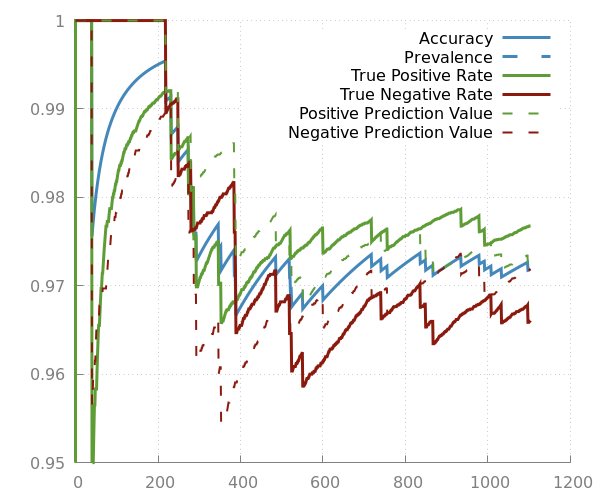
\includegraphics[scale=0.3]{img/output_run_0_confusion_matrix_1.png}
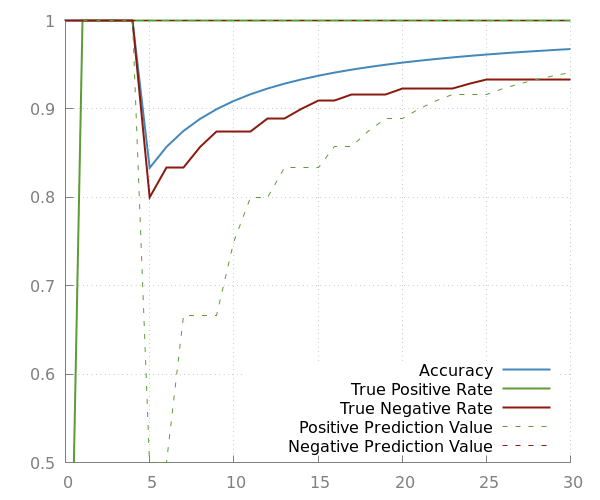
\includegraphics[scale=0.3]{img/splice_output_run_0_confusion_matrix_1.png}
\caption{Evolution of the confusion matrix during the prediction phase for \texttt{phishing} and \texttt{splice} datasets.}
\label{fig:evolution_phishing}
\end{figure}
The average confusion matrix obtained for each dataset is showed in Table \ref{table:confusion_matrix}. The performance indicators are reported in Table \ref{table:perf_indicators}. The proposed algorithm performs very well on a wide range of datasets as reported by \cref{table:confusion_matrix,table:perf_indicators}, in particular when they contain strong predictors as it is the case for \texttt{mushroom}. The accuracy is contained in a range from 0.8206 (\texttt{adult}) to 1 (\texttt{mushrooms}) while the $\text{F}_1$-score is bounded by 0.8653 (\texttt{heart}) and 1 (\texttt{mushrooms}). On \texttt{adult}, the accuracy is only 6\% higher than the prevalence, i.e. a baseline model consisting in returning 1 for any point would be only 6\% worse. This relatively poor performance in learning the underlying decision mapping is better reflected by the Matthews correlation coefficient of $0.51$.

By default, the false positives and false negatives are equilibrated for each dataset, despite a huge variation in the prevalence (between 20\% and 64\%, cf. Table \ref{table:confusion_matrix}) which may be a desirable property depending on applications. In addition, the results were obtained with non-balanced training sets which are known to be a problem for many machine learning algorithms \cite{He:2009:LID:1591901.1592322}. Moreover, the performance indicators remain stable during the whole prediction phase as shown by Figure \ref{fig:evolution_phishing} for the dataset \texttt{phishing} (similar result is observed for all datasets).

For a given case, the support is a metric of confidence in the prediction as illustrated in Figure \ref{fig:phishing_predictive_measure}. In general, the wrongly classified cases have a smaller difference between the evidence for each class which confirm the interest in the hyperparameters $\eta$ and $\bar \eta$ used in \eqref{eqn:updated_cr}. This can also be observed in Figure \ref{fig:phishing_histogram}.

\begin{figure}[!h]
\centering
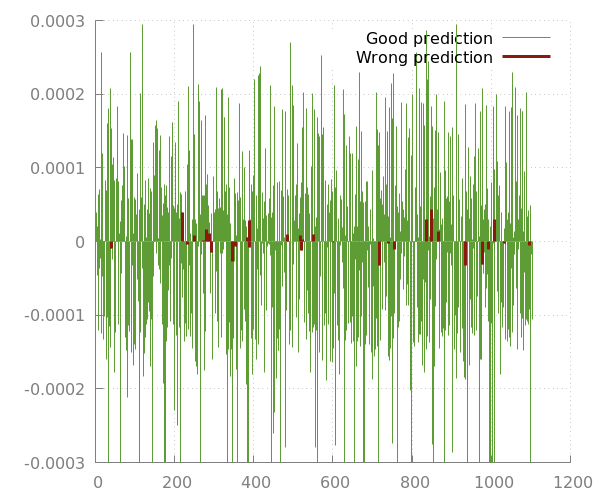
\includegraphics[scale=0.3]{img/output_run_0_diff_pred_1.png}
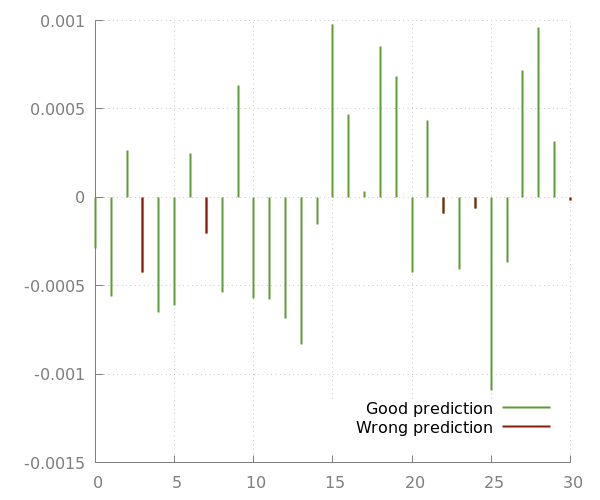
\includegraphics[scale=0.3]{img/output_run_2_diff_pred_1.png}
\caption{Difference between the weight assigned to both classes for each decision on \texttt{phishing} and \texttt{splice} (average). Similar results are observed for all datasets.}
\label{fig:phishing_predictive_measure}
\end{figure}

\begin{figure}[!h]
\centering
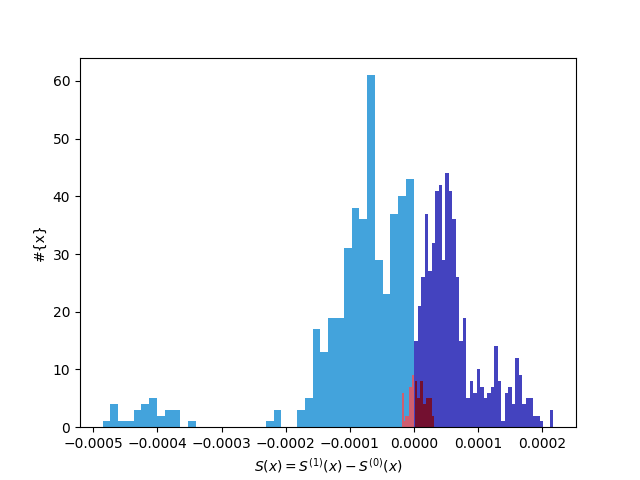
\includegraphics[scale=0.4]{img/phishing.png}
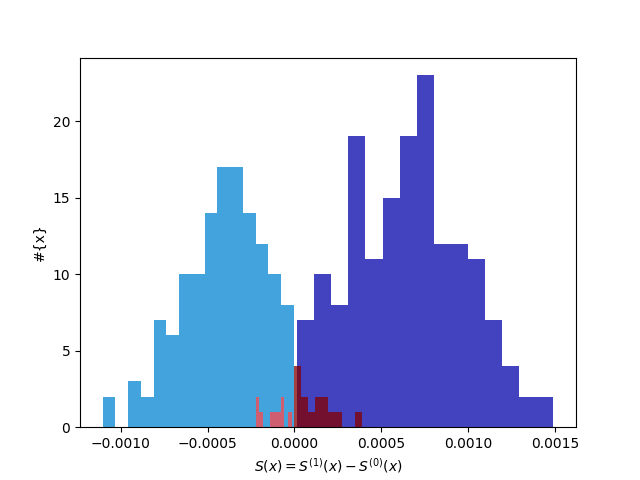
\includegraphics[scale=0.4]{img/splice.png}
\caption{Histogram of decisions depending on the strength for \texttt{phishing} and \texttt{splice}. In blue the correctly classified elements, in red the wrongly classified ones. The false positives and false negatives are concentrated around 0. Similar results are observed for all datasets.}
\label{fig:phishing_histogram}
\end{figure}

To compare the results of the proposed method, we explored the best results from the literature for each dataset.
The results are summarized in Table \ref{table:prev_results}. In \cite{doi:10.1504/IJBISE.2016.081590}, 5 rule-based classification techniques dedicated to medical databases are compared and achieve at best 95.85\% and 82.96\% accuracy resp. on \texttt{breast}, and \texttt{heart} datasets. Comparing bayesian approaches, \cite{Jiang:2012:LIW:2124637.2124641} demonstrated 97.35\% (\texttt{breast}) and 83.00\% (\texttt{heart}) accuracy. A 5 layers neural network with fuzzy inference rules achieved 87.78\% on \texttt{heart} \cite{sagir2017hybridised} while a k-NN algorithm reached 99.96\% on \texttt{mushrooms} \cite{Das:2001:FWB:645530.658297}. The best alternative among 6 rules-based classification methods achieved 95.84\% on \texttt{breast} and 100.00\% on \texttt{mushroom} \cite{HADI2017287}. Using 80\% of \texttt{phishing} as training set, an adaptative neural network achieved an average accuracy of 93.76\% (among 6 alternatives) with the best run at 94.90\% \cite{7727750}. Still on \texttt{phishing}, \cite{7881507} proposes to combine several classifiers and reaches 97.75\% accuracy for the best hybrid model (and demonstrates 97.58\% for Random Forest classifier). On \texttt{adult}, the comparison of several classifiers (naive bayes, decision tree, ...) demonstrated at most 86.25\% accuracy \cite{kou2012evaluation} while a Support Vector Machine approach reached 85.35\% \cite{Lee2001}. On \texttt{splice}, a method using Fuzzy Decision Trees \cite{5409447} reaches 94.10\% accuracy and a neural network combined to boosting \cite{catak2017} 97.54\%. On \texttt{breast}, Support Vector Machine approaches reached resp. 96.87\%, 98.53\%, 99.51\% accuracy \cite{CHEN20119014, POLAT2007694, akay2009support}, 99.26\% and 97.36\% for neural network based techniques \cite{MARCANOCEDENO20119573, ubeyli2007implementing}, 98.1\% for a bayesian network method \cite{fallahi2011expert}, or 94.74\% using Decision Trees \cite{quinlan1996improved}. On \texttt{skin}, \cite{catak2017} reports 98.94\% accuracy against 99.68\% for Decision Tree based method~\cite{6627823}. The best result, as far as we know, is 99.92\%, obtained by a Generalized Linear Model~\cite{basterrech2015generalized} (with 80\% training set).

The accuracy is slightly lower than the best results from the literature (\texttt{adult} 82.06\% against 86.25\%, \texttt{breast} 96.96\% against 99.51\%, \texttt{heart} 85.77\% against 87.78\%, \texttt{phishing} 96.05\% against 97.75\%, \texttt{splice} 94.43\% against 97.54\%, \texttt{skin} 98.65\% against 99.92\%). We explain this by at least two factors. First, the best methods on a given dataset are often dedicated to this dataset with {\it ad-hoc} or engineered parts which is not the case of \HCBR. Secondly, the hyperparameter familly $\eta$ have not been tuned but as we will show in next section, they might have a decisive impact on performance.
\HCBR~ performed better than Bayes classifier in two thirds of cases. Bayes classifier performs better on \texttt{breast} by approximately 1\% which represents less than one case wrongly classified. Similar results are observed with Decision Trees. However, the 1\% difference on \texttt{skin} represents an average of 7 cases misclassified in comparison in favor of Bayes. It performs better than Rule-based approaches (or gives similar results on \texttt{mushrooms} with an accuracy of 1) in the four considered references on three different datasets. Notice that combined with Neural Network, Rule-based achieves the state-of-art result on \texttt{heart} dataset. Except for \texttt{phishing}, Neural Network returns better results ($0.46$ more cases with correct classification in average for \texttt{breast}, $71$ for skin and almost $10$ for \texttt{splice}). Last, SVM gives better results in all three cases, but appear only as best results in two datasets.

Even if \HCBR~ does not rank first, we see at least three reasons to use it in practice. First, it provides consistently good results on all datasets without a need to tune the hyperparameters (which will be confirmed with the second round of experiments below), without using stratified sample to correct the unbalanced datasets or feature transformation that would require expert knowledge. In other words, it requires absolutely no domain knowledge or data science experience to deploy and use. Second, \HCBR~ works directly on unstructured dataset without a need of some exotic representations or encoders as it is the case for other methods. This has a considerable advantage in practice where the information per case is rarely structured by default. Last but not least, \HCBR~ provides local explanation: for each case and each group of features $\mathbf e_i$ in this case, \HCBR~ provides not only the support for $\mathbf e_i$ but also all the cases that participated in increasing the support. In the medical domain, the practitioner may check for instance the top two groups of features and for each the five most influencing past cases to find a reasonable justification to the prediction.

\begin{table}[h!]
\begin{center}
  \caption{Average confusion matrix obtained with a 10-fold cross-validation.}
 %\resizebox{12cm}{!}{
  \begin{small}
  \begin{tabular}{|l|c|c|c|c|c|c|c|c|c|c|c|}
    \hline
     & TP & FN & FP & TP & Prevalence\\
    \hline
    \texttt{adult} & 2182.40 & 295.30 & 288.50 & 488.80 & 0.7586\\
    \texttt{breast} & 23.00 & 1.40 & 0.70 & 43.90 & 0.3338\\
    \texttt{heart} & 12.40 & 1.80 & 1.90 & 9.90 & 0.5107\\
    \texttt{mushrooms} & 390.60 & 0.00 & 0.00 & 420.40 & 0.4804\\
    \texttt{phishing} & 595.40 & 23.80 & 19.80 & 465.00 & 0.5562\\
    \texttt{skin} & 4886.30 & 132.40 & 199.40 & 19286.90 & 0.2075\\
    \texttt{splice} & 155.70 & 9.10 & 8.50 & 142.70 & 0.5164\\
    \hline
  \end{tabular}
  \end{small}
  %}
  \label{table:confusion_matrix}
\end{center}
\end{table}
\begin{table*}[htbp]
\begin{center}
  \caption{Average performances obtained with a 10-fold cross-validation.}
 \resizebox{16cm}{!}{
  \begin{small}
  \begin{tabular}{|l|c|c|c|c|c|c|c|c|c|c|c|}
    \hline
     & Accuracy (std dev.) & Recall & Specificity & Precision & Neg. Pred. Value & $\text{F}_1$ score & MCC\\
    \hline
    \texttt{adult} & 0.8206 (0.0094) & 0.8832 & 0.6233 & 0.8808 & 0.6290 & 0.8820 & 0.5081\\

    \texttt{breasts} & 0.9696 (0.0345) & 0.9691 & 0.9676 & 0.9479 & 0.9844 & 0.9575 & 0.9344\\
    \texttt{heart} & 0.8577 (0.0943) & 0.8695 & 0.8437 & 0.8699 & 0.8531 & 0.8653 & 0.7178\\
    \texttt{mushrooms} & 1.0000 (0.0000) & 1.0000 & 1.0000 & 1.0000 & 1.0000 & 1.0000 & 1.0000\\
    \texttt{phishing} & 0.9605 (0.0081) & 0.9680 & 0.9514  & 0.9615 & 0.9590 & 0.9647 & 0.9199\\
    \texttt{skin} & 0.9865 (0.0069) & 0.9608 & 0.9932  &0.9736 & 0.9898 & 0.9672 & 0.9587 \\
    \texttt{splice} & 0.9443 (0.0124) & 0.9478 & 0.9398 & 0.9450 & 0.9441 & 0.9463 & 0.8884\\
    \hline
  \end{tabular}
  \end{small}
  }
  \label{table:perf_indicators}
\end{center}
\end{table*}
\begin{table}[h!]
\begin{center}
  \caption{Previous literature results measured as the highest accuracy obtained by the authors.}
  %\resizebox{12cm}{!}{
  \begin{small}
\begin{tabular}{|c|c|l|c|}
\hline
 Dataset & Ref. & Type & Accuracy   \\ \hline
\multirow{2}{*}{\texttt{adult}} & \cite{kou2012evaluation} & Many classifiers &  86.25\% \\
& \cite{Lee2001} & SVM & 85.35\% \\ 
& & \bfHCBR & {\bf 82.06\%} \\ \hline
 \multirow{10}{*}{\texttt{breast}} & \cite{akay2009support}  & SVM & 99.51\% \\ 
 & \cite{MARCANOCEDENO20119573} & Neural Net & 99.26\% \\ 
 & \cite{POLAT2007694} & SVM & 98.53\% \\ 
 & \cite{fallahi2011expert} & Bayes & 98.1\% \\ 
 & \cite{ubeyli2007implementing} & Neural Net & 97.36\% \\ 
 & \cite{Jiang:2012:LIW:2124637.2124641} & Bayes & 97.35\% \\ 
 & & {\bf \bfHCBR} & {\bf 96.96\%} \\
 & \cite{CHEN20119014} & SVM & 96.87\% \\
 & \cite{doi:10.1504/IJBISE.2016.081590} & Rule-based & 95.85\% \\
 & \cite{HADI2017287} & Rule-based & 95.84\% \\
 & \cite{quinlan1996improved} & Decision Tree & 94.74\% \\ \hline
 \multirow{3}{*}{\texttt{heart}} & \cite{sagir2017hybridised} & Neural Network + Rule-based & 87.78\%\\
 & & {\bf \bfHCBR} & {\bf 85.77\%} \\
 & \cite{Jiang:2012:LIW:2124637.2124641} & Bayes & 83.00\% \\ 
 & \cite{doi:10.1504/IJBISE.2016.081590} & Rule-based & 82.96\% \\ \hline
 \multirow{2}{*}{\texttt{mushrooms}} &  \cite{HADI2017287} & Rule-Based & 100.00\% \\ 
  & & {\bf \bfHCBR} & {\bf 100.00\%} \\
  & \cite{Das:2001:FWB:645530.658297} & k-NN & 99.96\% \\ \hline
 \multirow{3}{*}{\texttt{phishing}} & \cite{7881507} & Ensemble & 97.75\% \\ 
 &  \cite{7881507} & Random-Forest & 97.58\% \\ 
 & & {\bf \bfHCBR}& {\bf  96.05\%} \\
 & \cite{7727750} & Neural Net &  94.90\% \\\hline
 \multirow{3}{*}{\texttt{skin}} & \cite{basterrech2015generalized} & Generalized Linear Model & 99.92\% \\ 
 & \cite{6627823} & Decision Tree & 99.68\% \\ 
 & \cite{catak2017} & Neural Network + Boosting & 98.94\% \\
 & & {\bf \bfHCBR} & {\bf 98.65\%} \\ \hline
 \multirow{2}{*}{\texttt{splice}} & \cite{catak2017} & Neural Network + Boosting & 97.54\% \\
 & & {\bf \bfHCBR} & {\bf 94.43\%} \\
 & \cite{5409447} & (fuzzy) Decision Tree & 94.10\% \\ \hline
\end{tabular}
\end{small}
  %}
  \label{table:prev_results}
\end{center}
\end{table}

\subsubsection{Robustness comparison}

As mentionned above, the state-of-art results obtained per database required a lot of efforts in terms of feature selection and transformation, as well as model selection or hyperparameter tuning. Therefore, the obtained models are slightly better than \HCBR~ but not well adapted to solve several instances of the classification problem. If well-calibrated models with high performances on their domain of application is undeniably useful for practical usage, being able to solve a problem on a large variety of instances without effort is also of a vital importance, especially in the industry where the end-user might not be specialized in data science and machine learning. One main challenge of large scale machine learning systems is thus to achieve this good compromise between ready-to-deploy models and good performance metrics. With this perspective, comparing the state-of-art result per instance might not be a good indicator of this scalability capacity of a particular method. 

For a fair comparison, we performed a 10 cross-validation for each of the 7 selected datasets using 9 standard classification methods: AdaBoost, k-Nearest Neighbors, Linear SVM, Radius-Based Function (RBF) SVM, Decision Tree, Random Forest, Neural Network and Quadratic Discriminant Analysis (QDA). The implementation is provided by Scikit-Learn \cite{scikit-learn}. No hyperparameter tuning was performed and the default values of parameters were used.
Matthew Correlation Coefficient has been shown to be more informative than other metrics derivated from the confusion matrix \cite{Chicco2017}, in particular with unbalanced datasets. For this reason, we used it instead of the accuracy or $F_1$ score and reported the MCC per dataset as well as the average MCC and the corresponding rank (see Table \ref{table:scikit_results}). Additionally, we displayed the evolution of MCC with the training set size in Figure \ref{fig:mcc_by_examples}. 

The highest MCC value is obtained by Neural Network with 0.8914 followed by \HCBR~ with 0.8435. Neural Network improves \HCBR~ result by 5.68\% while \HCBR~ improves the result of all other methods from 2\% to 17.56\%. The lowest MCC score is obtained by Naive Bayes with 0.6953, mostly because it performs poorly on some datasets (0.2493 on \texttt{adult}, 0.5292 on \texttt{phishing} or 0.7600 on \texttt{skin}). In general, Neural Network and \HCBR~ are the only two methods whose rank remains consistent across all datasets, close to the first and second rank. On the contrary, methods like $k$-Nearest Neighbors or Decision Tree performed very well on one dataset (\texttt{skin}, resp. \texttt{splice}). Surprisingly, Random Forest not only perform poorer than Decision Tree but also performs worse than most methods. 
Naive Bayes and QDA perform very poorly in general which is less surprising knowing the assumptions behind those methods that are likely to be unrealistic on real datasets.

In other words, \HCBR~ and Neural Network have shown to be more versatile than the other approaches on this selected set of classification instances and without parameter tuning. We have no doubt that the results obtained with other methods can be highly improved by a proper hyperparameter selection, in particular for Random Forest or even k-Nearest Neighbors.

\begin{table}[h!]

  \caption{Comparison of \HCBR~ with several methods (Scikit-Learn implementation). }
  %\resizebox{12cm}{!}{
  \begin{minipage}{.5\linewidth}
\fontsize{10pt}{12pt}\selectfont 
\begin{tabular}{|c|l|l|c|}
\hline
 Dataset & Method & MCC & \#  \\ \hline

\multirow{10}{*}{\texttt{adult}} & \bfHCBR & 0.5146 & 3 \\
& AdaBoost & 0.5455  & 1 \\
& k-NN & 0.4785 & 7 \\
& Linear SVM & 0.4918 & 5\\
& RBF SVM & 0.5065 & 4\\
& Decision Tree & 0.4821  & 6\\
& Rand. Forest & 0.3776 & 8 \\
& Neural Net & 0.5349  & 2 \\
& Naive Bayes & 0.2493 & 9\\
& QDA & 0.4785  & 7 \\ \hline

\multirow{10}{*}{\texttt{breast}} & \bfHCBR & 0.9222 & 3 \\
& AdaBoost & 0.9023 & 6\\
& k-NN & 0.9163 & 4\\
& Linear SVM & 0.9126 & 5\\
& RBF SVM & 0.8829 & 8\\
& Decision Tree & 0.8760 & 9\\
& Rand. Forest & 0.9296 & 1\\
& Neural Net & 0.9280 & 2\\
& Naive Bayes & 0.8991 & 7\\
& QDA & 0.8616 & 10\\ \hline

\multirow{10}{*}{\texttt{heart}} & \bfHCBR & 0.7082 & 1 \\
& AdaBoost & 0.5972  & 6\\
& k-NN & 0.5879 & 7\\
& Linear SVM & 0.6849 & 4\\
& RBF SVM & 0.6287 & 5 \\
& Decision Tree & 0.5763  & 8\\
& Rand. Forest &0.5703 & 9\\
& Neural Net & 0.6995 & 2\\
& Naive Bayes & 0.6932 & 3\\
& QDA & 0.4500 & 10 \\ \hline

\multirow{10}{*}{\texttt{mushrooms}} & \bfHCBR & 0.9995 & 2 \\
& AdaBoost & 1.0000 & 1\\
& k-NN & 0.9993 & 3\\
& Linear SVM & 1.0000 & 1\\
& RBF SVM & 0.9990 & 5\\
& Decision Tree &  0.9991& 4\\
& Rand. Forest & 0.8840  & 7\\
& Neural Net &1.0000 & 1\\
& Naive Bayes & 0.9767 & 6\\
& QDA & 1.0000 & 1\\ \hline

\end{tabular}
\end{minipage}%
    \begin{minipage}{.5\linewidth}
\fontsize{10pt}{12pt}\selectfont 
\begin{tabular}{|c|l|l|c|}
\hline
 Dataset & Method & MCC & \#  \\ \hline

\multirow{10}{*}{\texttt{phishing}} & \bfHCBR & 0.9191 &  1\\
& AdaBoost & 0.8637 & 6\\
& k-NN & 0.9138 & 4\\
& Linear SVM & 0.8740 & 5\\
& RBF SVM & 0.9286 & 2\\
& Decision Tree & 0.8585 & 7\\
& Rand. Forest & 0.7582 & 8\\
& Neural Net & 0.9448 & 1\\
& Naive Bayes & 0.5292 & 10\\
& QDA & 0.5872 & 9\\ \hline

\multirow{10}{*}{\texttt{skin}} & \bfHCBR & 0.9551 & 4 \\
& AdaBoost & 0.8552 & 8\\
& k-NN & 0.9982 & 1 \\
& Linear SVM & 0.8090 & 9\\
& RBF SVM & 0.9950 & 3 \\
& Decision Tree & 0.9544 & 5\\
& Rand. Forest & 0.9539 & 6\\
& Neural Net & 0.9967 & 2\\
& Naive Bayes & 0.7600 & 10\\
& QDA & 0.9483 & 7\\ \hline

\multirow{10}{*}{\texttt{splice}} & \bfHCBR & 0.8857 & 2 \\
& AdaBoost & 0.8801 & 3\\
& k-NN & 0.6072 & 9\\
& Linear SVM & 0.7282 & 8\\
& RBF SVM & 0.8461 & 4 \\
& Decision Tree & 0.8998 & 1\\
& Rand. Forest & 0.5925 & 10\\
& Neural Net & 0.8390 & 5\\
& Naive Bayes & 0.7595 & 7\\
& QDA & 0.8251 & 6\\ \hline
\end{tabular}
\end{minipage}
  %}
  \label{table:prev_results}
\end{table}

\begin{table}[h!]
\begin{center}
  \caption{Average MCC and rank obtained with several methods (Scikit-Learn implementation). The column $\Delta_{\HCBR}$ represents the relative difference in MCC w.r.t. to \HCBR.}
  %\resizebox{12cm}{!}{
  \begin{small}
\begin{tabular}{|l|c|c|r|}
\hline
  Method & MCC & Rank & $\Delta_{\HCBR}$ \\ \hline
 
 Neural Network & 0.8914 & 1 & 5.68\%\\
 \bfHCBR & 0.8435 & 2 & - \\
 RBF SVM & 0.8267 & 3 & 2.00\%\\
 Decision Tree & 0.8066& 4 & 4.37\% \\
 AdaBoost & 0.8063 & 5 & 4.41\% \\
 k-NN & 0.7859 & 6 & 6.82\% \\
 Linear SVM &  0.7858 & 7 & 6.84\% \\
 QDA & 0.7358 & 8 & 12.76\% \\
 Random Forest & 0.7237 & 9 & 14.20\% \\
 Naive Bayes & 0.6953 & 10 & 17.56\% \\
 \hline
\end{tabular}
\end{small}
  %}
  \label{table:scikit_results}
\end{center}
\end{table}




\begin{figure}[!h]\centering
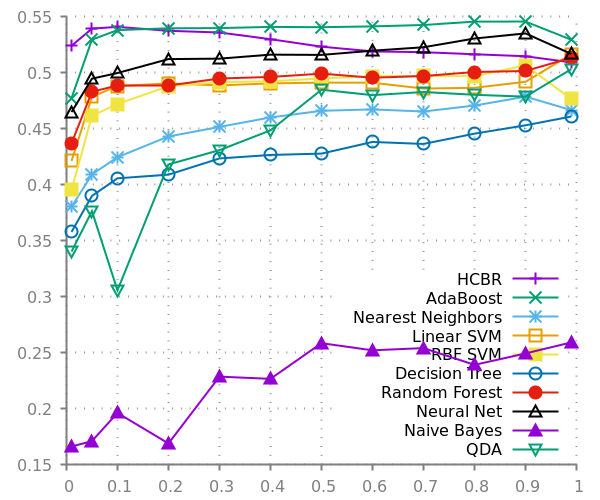
\includegraphics[scale=0.2]{img/mcc_by_examples_adult.png}
\hfill
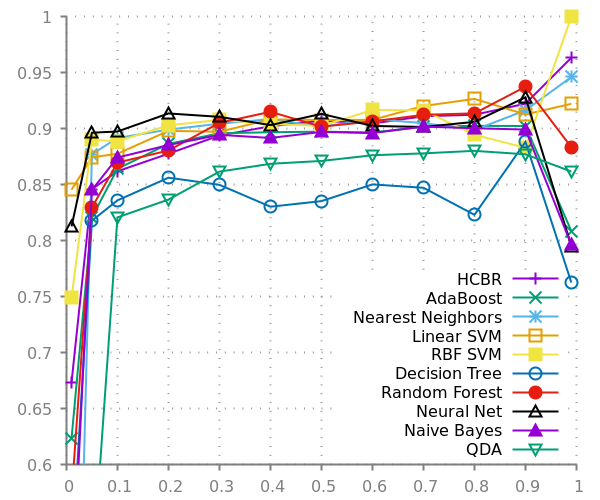
\includegraphics[scale=0.2]{img/mcc_by_examples_breast.png}
\hfill
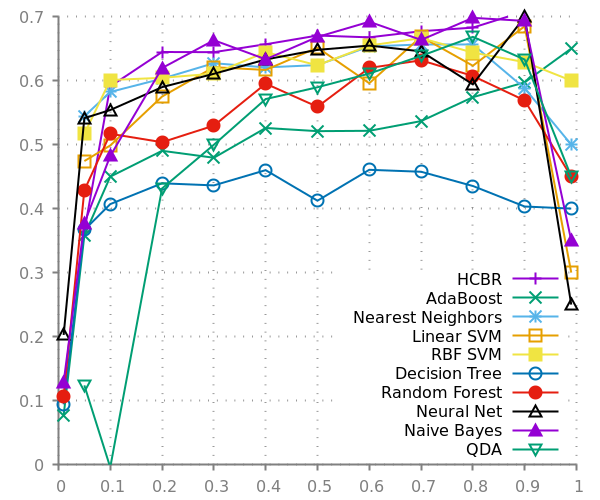
\includegraphics[scale=0.2]{img/mcc_by_examples_heart.png}
\hfill
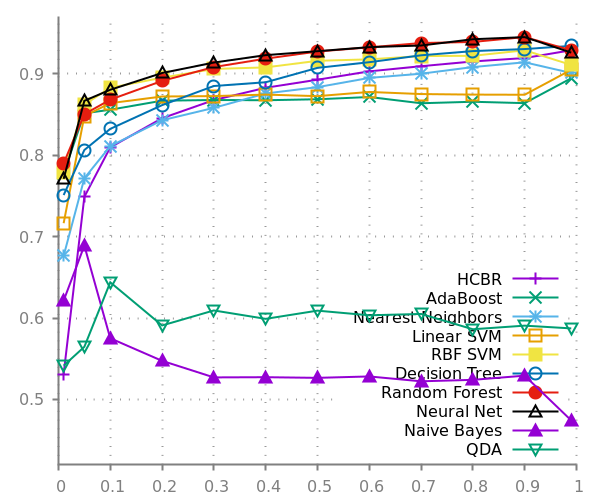
\includegraphics[scale=0.2]{img/mcc_by_examples_phishing.png}
\hfill
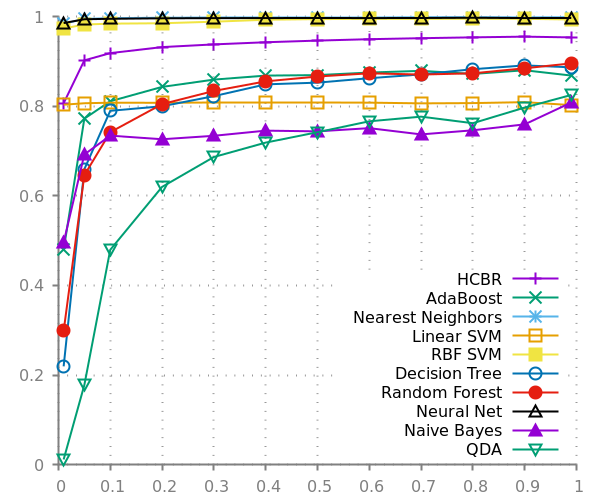
\includegraphics[scale=0.2]{img/mcc_by_examples_skin.png}
\hfill
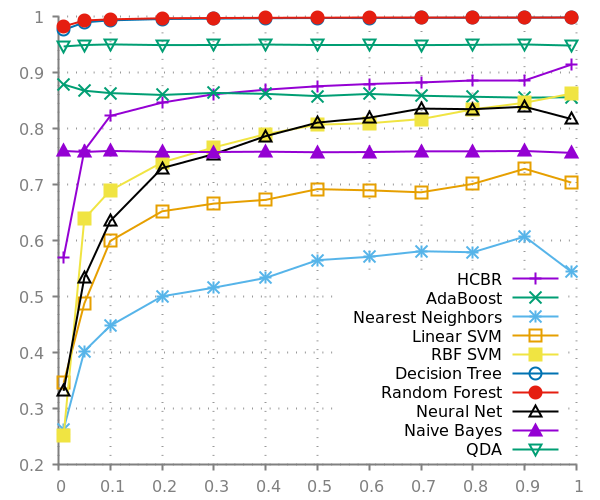
\includegraphics[scale=0.2]{img/mcc_by_examples_splice.png}
\caption{Matthew Correlation Coefficient depending on the training set size for \texttt{adult}, \texttt{breast},  \texttt{heart},  \texttt{phishing},  \texttt{skin} and  \texttt{splice}. The fitness is lower than the MCC by definition of \eqref{eq:opti_MCC}.}
\label{fig:mcc_by_examples}
\end{figure}



\subsection{Intrinsic performance}
\label{sec:intrinsic_perf}

In this section, we validate the time complexity and discuss the model space limitations of \HCBR. We also study the influence of the two main parameters (number of examples and size of the examples) on the computation time.\\

\subsubsection{Computation Time} We generated a casebase of $N$ cases of size $m$ such that case $i$ is described by $\{i, ...,  i+m\}$ i.e., each case is partitioned into $m$ elements (one discretionary feature). This is the worst-case scenario in terms of the size of $\mathcal{E}$ if $m < N$ because the family grows exponentially in function of $m$ or $N$. We split the computation time into constructing the hypergraph (and determining the intersection family) and calculating the strength of the partition. The results are illustrated in Figure \ref{fig:time}. By increasing $N$ with a fixed $m$, the partition grows exponentially and thus, it is expected to have an exponential curve for the strength computation. On the contrary, building the hypergraph can be done in linear time when $m$ fixed. When $N$ is fixed and $m$ increases, constructing the hypergraph is still doable in linear time as expected. Interestingly, calculating the strength has two phases: if $m \leq N$, increasing $m$ exponentially increases the time (because $\mathcal{E}$ exponentially increases) but if $m > N$, increasing $m$ cannot results in an exponential growth in the computation time (because $\mathcal{E}$ grows linearly).

\begin{figure}[!h]
\centering
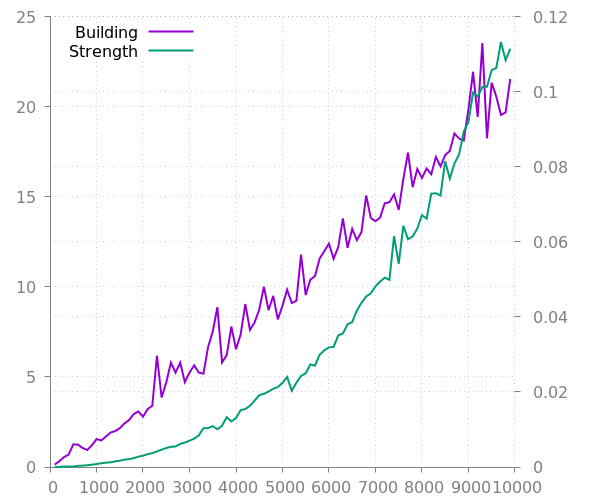
\includegraphics[scale=0.3]{img/time_k.png}
\hfill
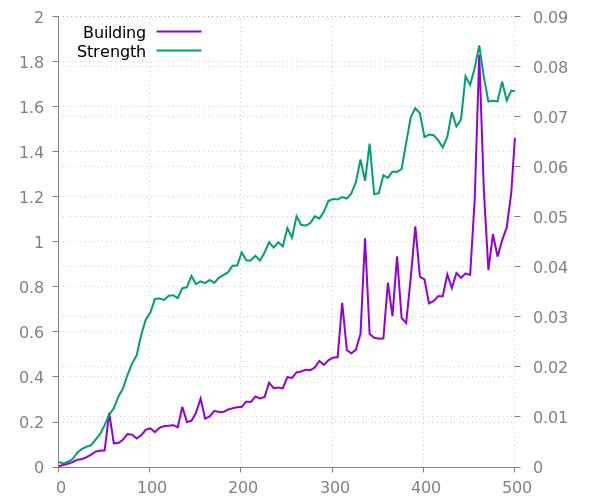
\includegraphics[scale=0.3]{img/time_n_old.png}
\caption{At the top, computation time to build the model (hypergraph construction + strength calculation) depending on $N$ ($m = 10$), and at the bottom, depending on $m$ ($N = 100$). The case $i$ is described by $\{i, ...,  i+m\}$ such that each case is partitionned into $m$ elements (one discretionary feature). Right scale for bulding and left scale for strength.}
\label{fig:time}
\end{figure}

\subsubsection{Learning Curves} The learning curves are useful to study the limit of the model space on the different datasets. It consists in plotting the accuracy in function of the training set size for both the predictions over the training and the test sets. For the training set, it is expected to observe an accuracy starting close to 1 and decreasing fast to reach a plateau. A low stationary accuracy value indicates a high bias in the model or/and an irreducible error contained in the dataset, such as noisy or uninformative features. Oppositely, the accuracy on the test sets starts close to 0 as the training set is small and should increase until a plateau which is very often expected to be lower than of the training set. If the training set curve converges toward a much higher value than the test set curve, then the model has a large variance. In other words, to achieve a good bias-variance tradeoff, the accuracy of both curves should converges toward more or less the same value, expected as high as possible.



\begin{figure}[!h]
\centering
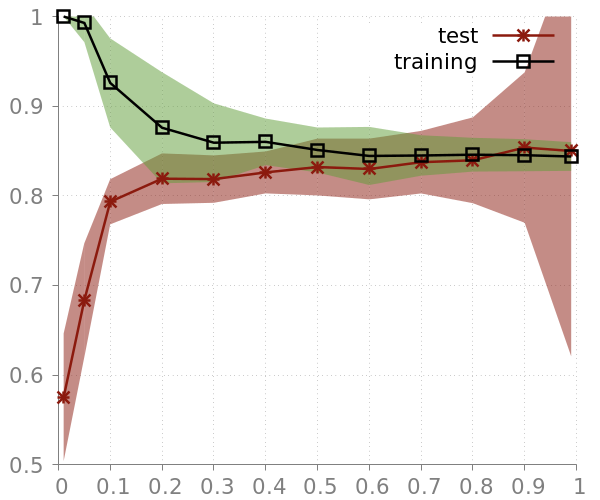
\includegraphics[scale=0.3]{img/learning_curve_heart.png}
\hfill
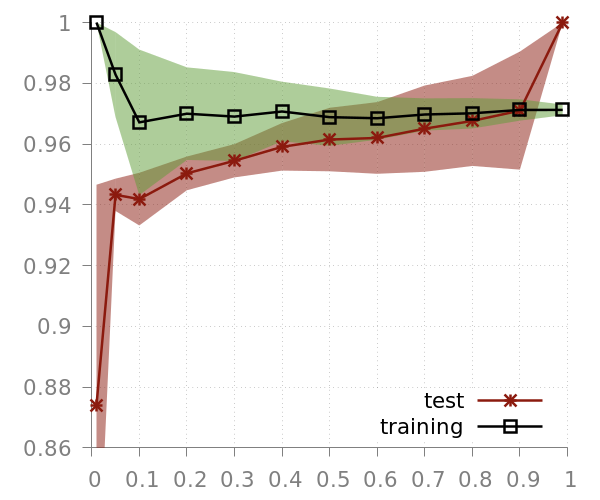
\includegraphics[scale=0.3]{img/learning_curve_breast.png}
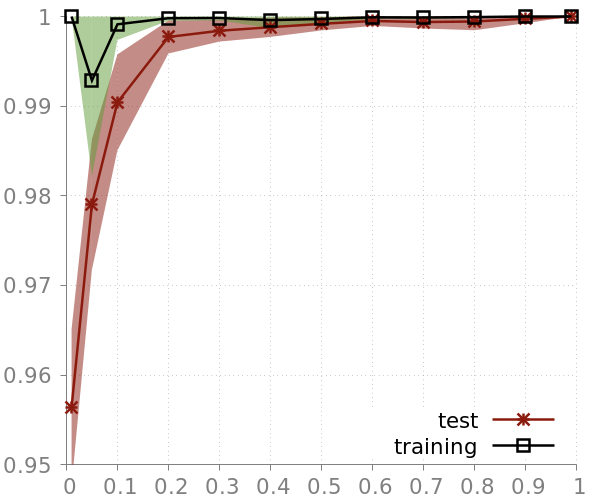
\includegraphics[scale=0.3]{img/learning_curve_mushrooms.png}
\hfill
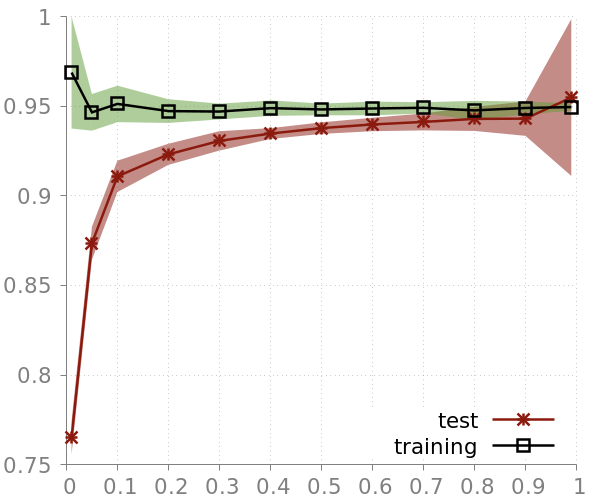
\includegraphics[scale=0.3]{img/learning_curve_splice.png}
\caption{Learning curves for \texttt{heart}, \texttt{breast}, \texttt{mushrooms} and \texttt{splice} datasets. Despite a bias and/or irreducible error observed on  \texttt{heart}, \texttt{breast} and \texttt{splice}, . The model variance appear very low on all datasets. Conversely, the bias and/or irreducible error ranges from very low on \texttt{mushrooms}, relatively low on \texttt{breast} and \texttt{splice} to high for \texttt{heart}.}
\label{fig:learning_curve_2}
\end{figure}

\begin{figure}[!h]\centering
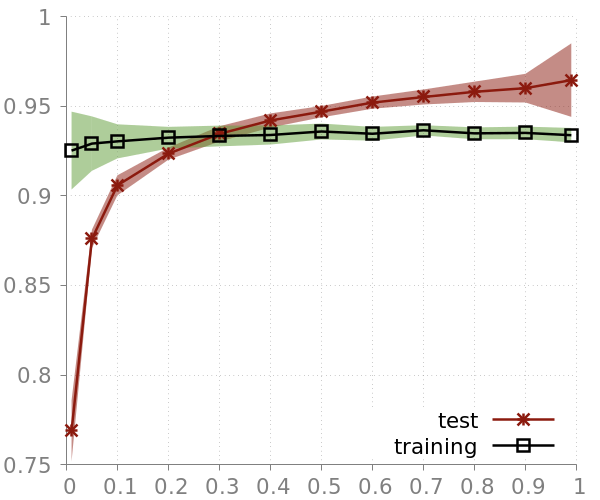
\includegraphics[scale=0.3]{img/learning_curve_phishing.png}
\hfill
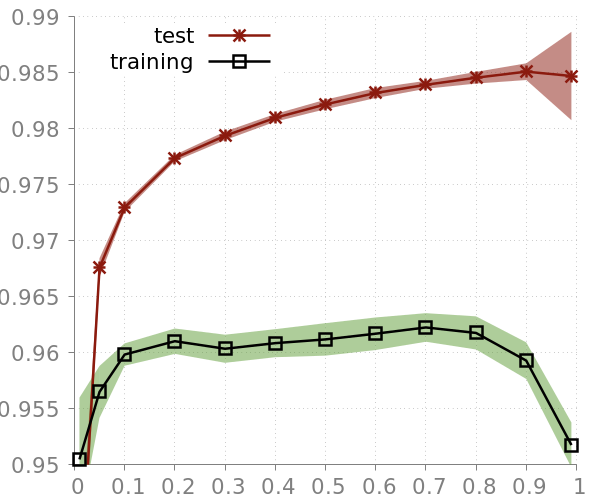
\includegraphics[scale=0.3]{img/learning_curve_skin.png}
\caption{Learning curves on \texttt{phishing} and \texttt{skin} datasets. The accuracy on the test set is higher than on the training set. On the training set, the accuracy starts by increasing and remaing globally stable (with a drop for \texttt{skin}).}
\label{fig:learning_curve_3}
\end{figure}


The learning curves are calculated as the average over 10 runs with random splits and are shown in Figures \ref{fig:learning_curve_1}, \ref{fig:learning_curve_2} and \ref{fig:learning_curve_3}. In addition, we displayed the variance of the 10 runs. The first remark concerns the variance. On all datasets, the variance is very low and the accuracy on the test set extremely close if not higher than those of the training set (see \texttt{phishing} and \texttt{skin} on \ref{fig:learning_curve_3}). Despite a relatively low accuracy, \HCBR~ seems to reach a good bias-variance compromise on \texttt{heart} suggesting a more complex model space might help. In general, the remark applies on the four datasets displayed in Figure \ref{fig:learning_curve_3} as the observed error rate results from bias and not only from irreducible error. Indeed, the literature comparison provided by Table \ref{table:prev_results} proves the accuracy could be improved.

The learning curves for \texttt{phishing} and \texttt{skin} are surprising for two reasons. First, the test accuracy is significantly higher than the training accuracy. Two reasons might have explained this: 1) we did not use stratified sample to rebalance the dataset, so if there is a difference in prevalence between the training set and test set, the model response might be different in favor of the test set and 2) the prediction phase on those two datasets uses an heuristic such that is a case is already in the casebase, the output must be similar to the one we know independantly of what the model predicts (i.e. we assume there is no noise in the outputs). For 1) a comparison of the performances indicators between the test set (see Table \ref{table:confusion_matrix}) and the training set (not shown for size reason) do not show any striking difference. Regarding 2), for both datasets, the difference in accuracy between the two curves is much higher than the possible gain due to the heuristic. The learning curves for the same experiment without the heuristic are display in Figure \ref{fig:learning_curve_4} and it seems to explain perfectly the phenomena. Notice that this is specific to those two datasets that contains several redundant points with the same output. For instance, the heuristic is activated also on \texttt{splice} but as the number of redundant elements is very low w.r.t. to the dataset size, the impact on the accuracy is not significant.
Secondly, we notice a significant drop in the training accuracy for large training set while the test accuracy remains stable. The fact the training accuracy starts relatively low is a statistical artifact due to the size of the training set as confirmed by the learning curve on very small training set (see Figure \ref{fig:learning_curve_5}).

Finally, the learning curve of \texttt{adult} in Figure \ref{fig:learning_curve_1} shows once again a small variance but high bias. Surprisingly, the accuracy slightly decreases with the training set size.

The analysis of the learning curves seems to indicate that the main limitation of \HCBR~ lies in a large bias. This may come either from the model space complexity or the model selection method that does not properly fit the parameters. The number of parameters in the model is equal to the cardinality of $\mu$, itself proportional to the number of atoms in the training set. However, a closer look at how a decision is taken reveal that each case has its own {\it small model} as a convex combination of its features. In other words, the real number of parameters to model the decision for a given case never exceed its number of features. This might not be enougth to represent fairely complex functions. To overcome this problem, we can extend the model space to include additional parameters and determine a method to infer their value from the training set. To discard the second hypothesis, we conducted additional investigations on the model selection in the next paragraph.


\begin{figure}[!h]\centering
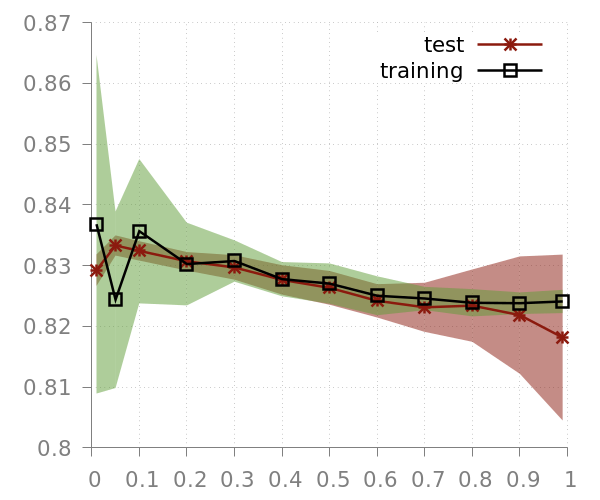
\includegraphics[scale=0.3]{img/learning_curve_adult.png}
\caption{Learning curve for \texttt{adult}.}
\label{fig:learning_curve_1}
\end{figure}

\begin{figure}[!h]\centering
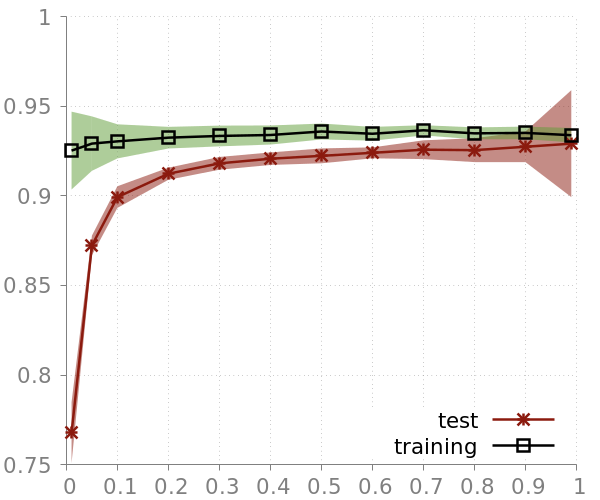
\includegraphics[scale=0.3]{img/learning_curve_phishing_no_heuristic.png}
\hfill
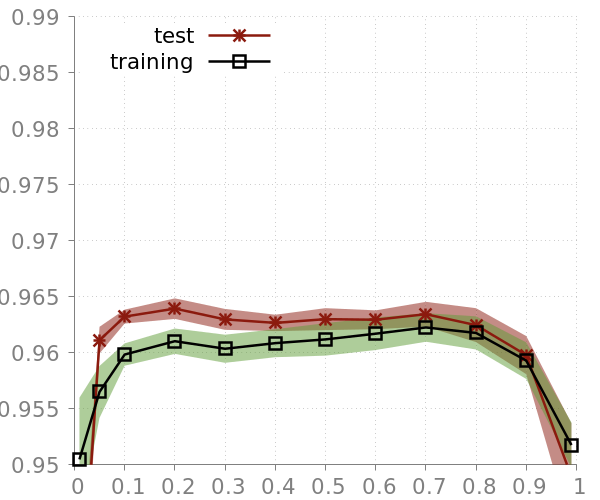
\includegraphics[scale=0.3]{img/learning_curve_skin_no_heuristic.png}
\caption{Learning curves on \texttt{phishing} and \texttt{skin} datasets without the heuristic. Compared to Figure \ref{fig:learning_curve_3}, the learning curve behave as expected in theory.}
\label{fig:learning_curve_4}
\end{figure}

\begin{figure}[!h]\centering
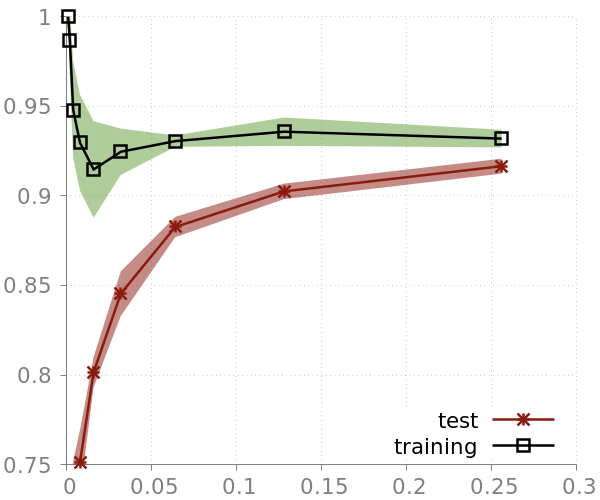
\includegraphics[scale=0.3]{img/learning_curve_phishing_zoom.png}
\hfill
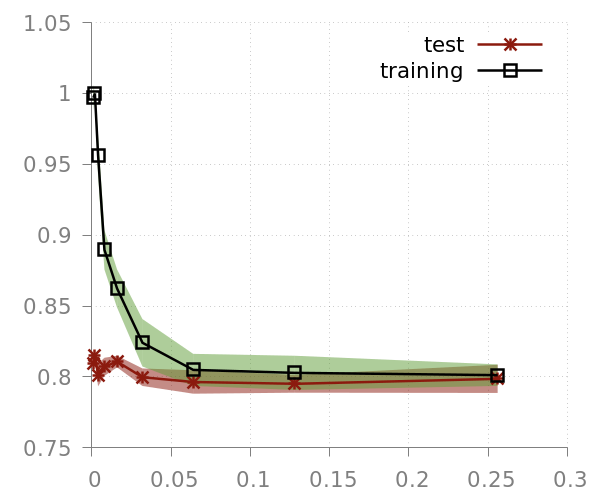
\includegraphics[scale=0.3]{img/learning_curve_adult_zoom.png}
\caption{Learning curves on \texttt{phishing} and \texttt{adult} for very small training set size.}
\label{fig:learning_curve_5}
\end{figure}

\subsubsection{Model Space limitation} We are interested in understanding whether it is possible for \HCBR~ to overfit the training set or at least improve the significantly the accuracy or MCC on the training set. We consider the matricial formulation of the support,
\begin{equation}
  S = W\mu
\end{equation}
and we are interested in knowing whether or not we can perturbate $\mu$ such that $S$ leads to classify correctly all the examples.% [TODO: NOTE ON SEPARABILITY]
As we already verified that the initial $\mu$ provides better results than baseline models, we would like to perturbate as little as possible $\mu$. For this, we calculate $\mathbf k$ such that $S + \mathbf k$ would correctly classify all the examples. We are looking for $\delta$ such that,

\begin{align}
 & S + \mathbf k  = W(\mu + \delta) \\
\Leftrightarrow & S + \mathbf k  = W\mu + W\delta \\
\Leftrightarrow & \mathbf k  = W\delta \\
\implies & \delta  = W^+ \mathbf k + [I - W^+W]\mathbf w, ~ \forall \mathbf w \in \mathbb{R}^N
\end{align}
with $W^+$ the Moore-Penrose pseudo-inverse of $W$. When $W$ is not of full rank, the solutions of the undertermined system are given for any vector $\mathbf w \in \mathbb{R}^N$, however, it can be shown that $\delta  = W^+\mathbf k$ is a least-square minimizer, i.e. $\forall \mathbf x \in \mathbb{R}^M ~ ||W\mathbf x -\mathbf k||_2 \geq ||W\delta - \mathbf k||_2$. In particular, if $||W\delta - \mathbf k||_2 = 0$, then all the elements would be correctly classified.

Of course, it might not be possible to obtain  $\delta$ such that $||W\delta - \mathbf k||_2 = 0$, but it does imply that there exist no couple $(\mathbf k, \delta)$ such that the accuracy is 1. Solving directly for all such couples seem to be a difficult problem without additional assumptions and thus, we adopted a slightly different approach: instead of fixing $\mathbf k$ a priori, we formulated the problem as optimizing the Matthew Correlation Coefficient:

\begin{equation}
\label{eq:opti_MCC}
\delta^* = \underset{\delta \in \mathbb{R}^M}{\max} ~ \text{MCC}(\delta, W) - c ||\delta||^2_2
\end{equation} where MCC is the Matthew Correlation Coefficient associated to $S = W \delta$ and $c$ a regularization factor. The regularization factor translates the idea that a smaller perturbation to obtain the same MCC is better than a larger one. We arbitrarily set $c$ to $0.1$. Despite further work could be needed to determine a more tailored value, the conclusions drawn from this section would remain valid.

To solve \eqref{eq:opti_MCC}, we used a $(\mu+\lambda)$ genetic algorithm with an evolution strategy. Each individual is made of two vectors: $\delta \in \mathbb{R}^M$ and a $\nu \in \mathbb{R}^M$ representing the mutation probability of each corresponding component of $\delta$. The mutation operator is a centered gaussian perturbation and the crossover a 2-points crossover. The implementation is provided by DEAP \cite{DEAP_JMLR2012}.


We performed 10 runs of a 10 folds cross-validation with random split and compared to the result obtained without the optimization process. The dataset \texttt{mushrooms} has been discarded as \HCBR~ reached an accuracy of 1. We set the population to 100, and for each dataset we adjusted the number of generations and the standard deviation of the gaussian mutation manually (see Table \ref{table:hyperparameters_ga}). To set the standard deviation of the mutation, we used $\sigma = \frac{\mu^-}{\alpha}$ where $\alpha$ is an empiracally determined factor and $\mu^-$ defined by $\underset{i,j}{\min}{~ \mu_i - \mu_j}$ i.e. the minimal difference between two components of $\mu$. The rational behind is that, once again, we would like to slightly perturbate $\mu$ and it is reasonable to think that a perturbation should be small enough not to directly switch the estimation of two elements of $\mu$. To conclude, we used a Wilcoxon signed-rank test at 5\% and 1\% on the test MCC obtained with and without the optimization process. There are three possible scenarios: 1) if the MCC can be improved on the training set and on the test set, it means the problem comes from the model selection method (estimation of $\mu$ and training) and results might be improved without changing the model space, 2) if the MCC can be improved on the training set but remains the same or deteriorate on the test set, the model space can represent the training set but overfit and thus should be extended 3) if the MCC cannot be improved even on the training set, then the model space is definitely not capable of representing properly the underlying decision mapping and should be extended.


A summary of the results are provided in Table \ref{table:opti_results} and the evolution of the fitness by Figure \ref{fig:fitness}. A look at Figure \ref{fig:fitness} confirms that the genetic algorithm converged or was closed to converged and was able to optimize the cost function. In all cases, the optimization procedure succeed to find a vector $\delta$ that yields a better MCC on the test sets. However, the improvement is quantiatively different from a dataset to another. For instance, on \texttt{heart} the absolute difference in MCC is 16\% (relative difference: 23.64\%) while on \texttt{phishing} the difference is barely 1\%. In general, the higher is the intial MCC and the less the improvement is visible. 

The variations of MCC on the test set are mitigated. The procedure returns significant changes in only two cases (\texttt{adult}) and (\texttt{skin}) for which one is improved (\texttt{adult}) and one deteriorated (\texttt{skin}). This seems to indicate that the model selection and training phase described in Section \ref{sec:model_selection} and \ref{sec:decision_training} returns one of the best MCC achievable within the model space. More precisely, the vector $\mu$ represents one of the best support approximation in its neighborhood. 


\begin{table}[h!]
\begin{center}
  \caption{Results obtained on solving \eqref{eq:opti_MCC}. The columns {\it initial MCC}, {\it $\Delta$ MCC training} and {\it$\Delta$ MCC test} represent respectively the initial MCC on the training set, the difference of MCC obtain on the training with and without the genetic algorithm, the difference of MCC obtain on the test sets with and without the genetic algorithm. {\it WSR r\%} indicates the result of the Wilcoxon signed-rank test at $r$\% risk (yes for significant difference in the sample median, no otherwise).}
  %\resizebox{12cm}{!}{
  \begin{small}
\begin{tabular}{|l|c|c|c|c|c|}
\hline
  Dataset & initial MCC & $\Delta$ MCC training & $\Delta$ MCC test & WSR 5\% & WSR 1\%\\ \hline
 \texttt{adult} &  0.5190 & 0.0400 & 0.0084 & yes & yes \\
  \texttt{breasts} & 0.9360 & 0.0312 & -0.0025 & no & no \\
  \texttt{heart} & 0.6912 & 0.1634 & -0.0023 & no & no  \\
    \texttt{phishing} & 0.8690 &0.0093 & 0.0002  & no & no  \\
    \texttt{skin} & & & -0.0118 &  yes & yes \\
    \texttt{splice} & 0.8866 & 0.0208 & 0.0006 & no & no  \\\hline
\end{tabular}
\end{small}
  %}
  \label{table:opti_results}
\end{center}
\end{table}


\begin{figure}[!h]\centering
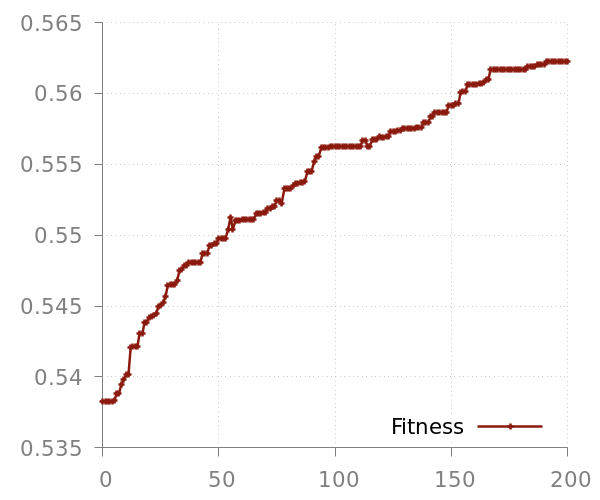
\includegraphics[scale=0.2]{img/fitness_mcc_adult.png}
\hfill
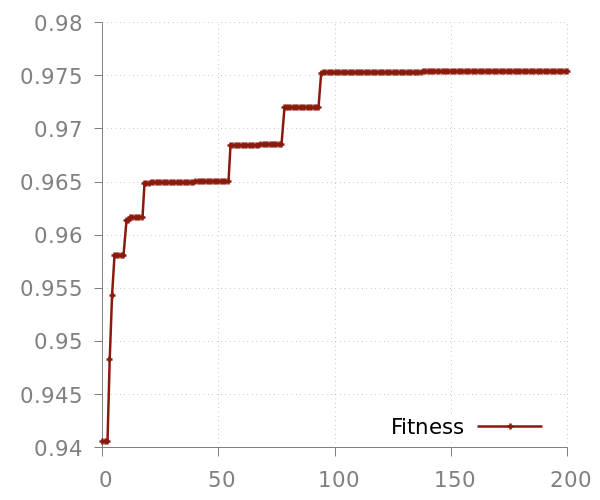
\includegraphics[scale=0.2]{img/fitness_mcc_breast.png}
\hfill
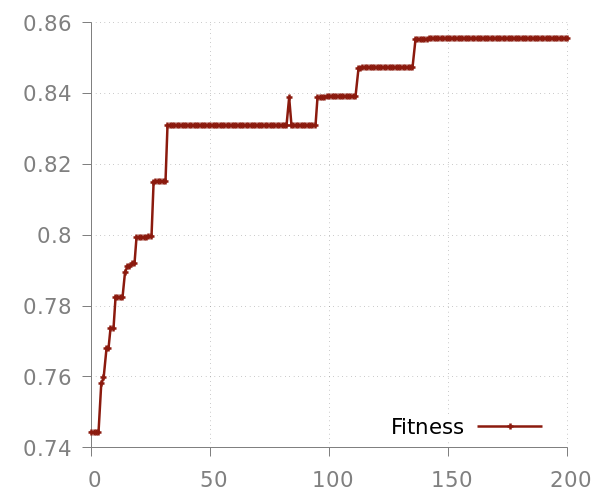
\includegraphics[scale=0.2]{img/fitness_mcc_heart.png}
\hfill
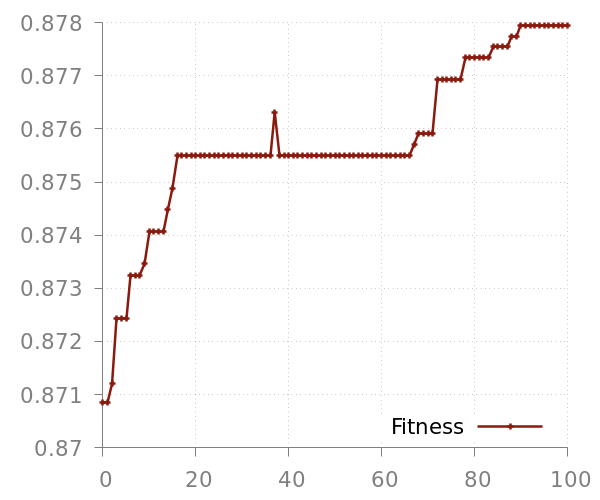
\includegraphics[scale=0.2]{img/fitness_mcc_phishing.png}
\hfill
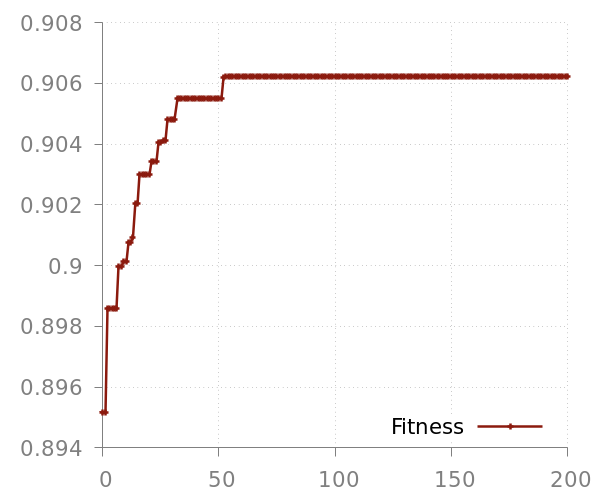
\includegraphics[scale=0.2]{img/fitness_mcc_splice.png}
\caption{Maximal fitness value in the population in function of generations for \texttt{adult}, \texttt{breast},  \texttt{heart},  \texttt{phishing},  \texttt{splice} and  \texttt{skin}. The fitness is lower than the MCC by definition of \eqref{eq:opti_MCC}.}
\label{fig:fitness}
\end{figure}


\begin{table}[h!]
\begin{center}
  \caption{Hyperparameters for the genetic algorithm. {\it Mutation $\sigma$ factor} is a factor used to set the standard deviation of the gaussian mutation. We use $\sigma = \frac{\mu^-}{\alpha}$ where $\alpha$ is the factor and $\mu^-$ defined by $\underset{i,j}{\min}{~ \mu_i - \mu_j}$.}
  %\resizebox{12cm}{!}{
  \begin{small}
\begin{tabular}{|l|c|c|}
\hline
  Dataset & Generations & Mutation $\sigma$ factor \\ \hline
 \texttt{adult} & 200 & 10000 \\
  \texttt{breasts} & 200 & 10 \\
  \texttt{heart} & 200 & 10 \\
    \texttt{phishing} & 100 & 1000 \\
    \texttt{skin} & 100 & 1000 \\
    \texttt{splice} & 200 & 100 \\\hline
\end{tabular}
\end{small}
  %}
  \label{table:hyperparameters_ga}
\end{center}
\end{table}

\subsubsection{Hyperparameters $\eta$} We used a 90-10 split and set $\eta_{-1} = \eta_1$ to ease the visualization. Instead of using the decision function defined by \eqref{eqn:decision_rule_revised}, we did not produce a prediction if the constraints $C_1$ or $C_0$ were not respected. It can be viewed as creating a third class {\it unknown} for which we consider we cannot produce a decision. We measured the accuracy and the test set size ratio for which a prediction has been produced for different values of $\eta := \eta_{-1} = \eta_1$. If $\bar J$ correctly approximates $J$, increasing $\eta$ should increase the accuracy while the test set ratio should remain high. Additionally, we plot the test set ratio in function of the accuracy and calculate the Pareto frontier\footnote{Points such that improving one component would degrades the other one.} which represents the best compromises accuracy/ratio. The closer the points are to $(1,1)$ the better it is. A Pareto frontier consisting of $(1,1)$ represents the perfect model (e.g. reached on \texttt{mushroom} dataset). Figures \ref{fig:meta_phishing}, \ref{fig:meta_breast}, \ref{fig:meta_heart} and \ref{fig:meta_adult} provides the result for the best and worst two datasets. Figure \ref{fig:meta_all} shows all of the four Pareto frontiers. 
\begin{figure}[!h]
\centering
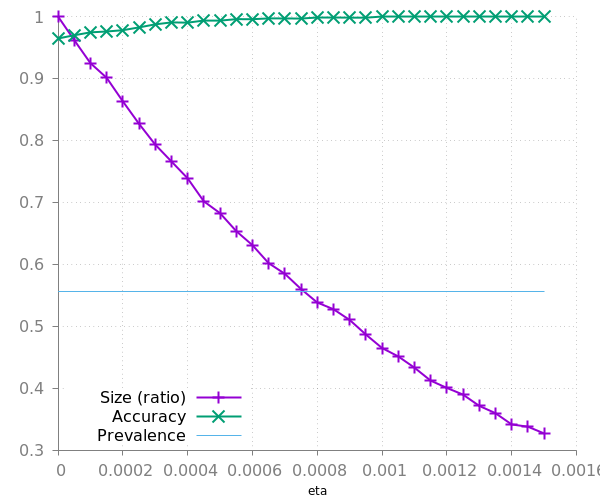
\includegraphics[scale=0.3]{img/meta_phishing.png}
\hfill
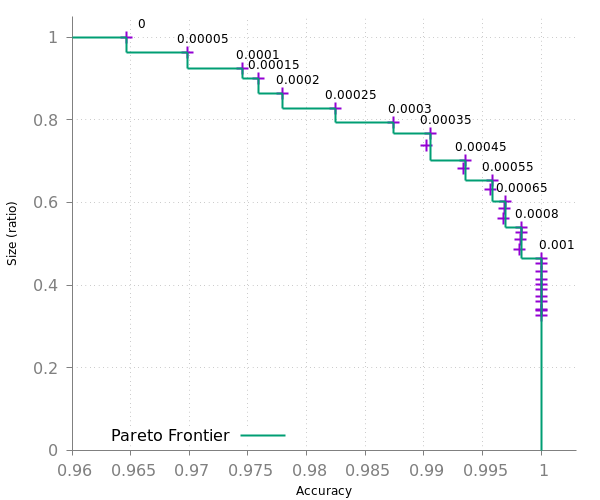
\includegraphics[scale=0.3]{img/meta_pareto_phishing.png}
\caption{Influence of $\eta$ on \texttt{phishing} dataset.}
\label{fig:meta_phishing}
\end{figure}
As expected, the results are better on \texttt{phishing} and \texttt{breast}. On \texttt{phishing}, \texttt{breast} and \texttt{heart}, the accuracy globally increases with $\eta$ while on \texttt{heart} the accuracy slightly decreases indicating poor influence of the hyperparameters and model. 

Notice that for certain values of $\eta$ it is possible to reach 100\% accuracy with \texttt{heart} while it is not with \texttt{breast}. Also, for high values of $\eta$, we observe a fall in accuracy for \texttt{breast}. We suspect those two phenomena to appear because we used the same value for $\eta_0$ and $\eta_1$. 

\begin{figure}[!h]\centering
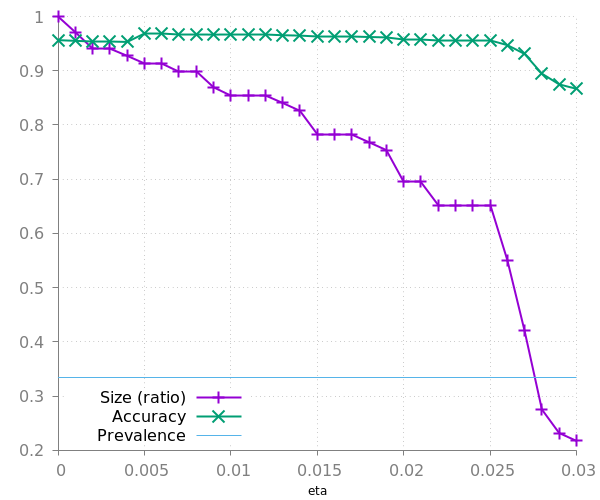
\includegraphics[scale=0.3]{img/meta_breast.png}
\hfill
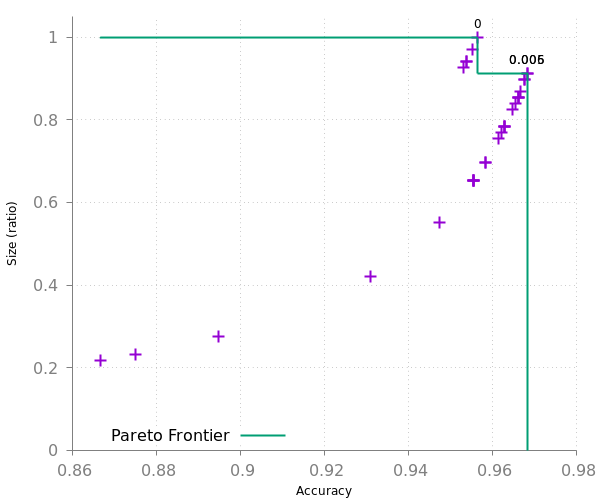
\includegraphics[scale=0.3]{img/meta_pareto_breast.png}
\caption{Influence of $\eta$ on \texttt{breast} dataset.}
\label{fig:meta_breast}
\end{figure}
\begin{figure}[!h]
\centering
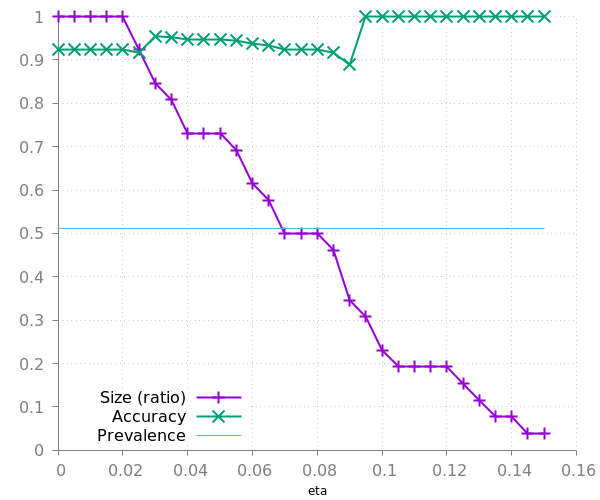
\includegraphics[scale=0.3]{img/meta_heart.png}
\hfill
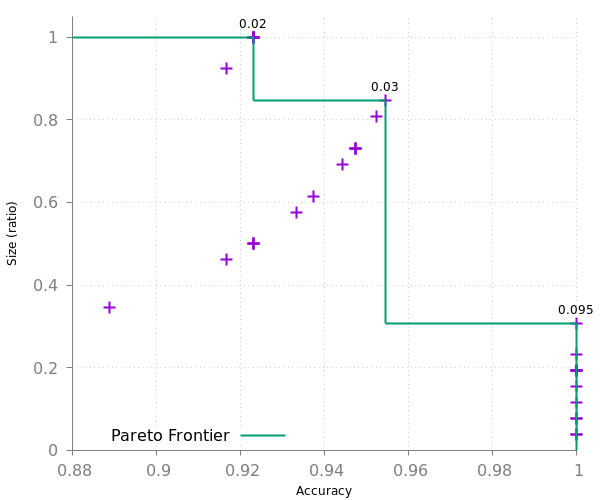
\includegraphics[scale=0.3]{img/meta_pareto_heart.png}
\caption{Influence of $\eta$ on \texttt{heart} dataset.}
\label{fig:meta_heart}
\end{figure}
\begin{figure}[!h]\centering
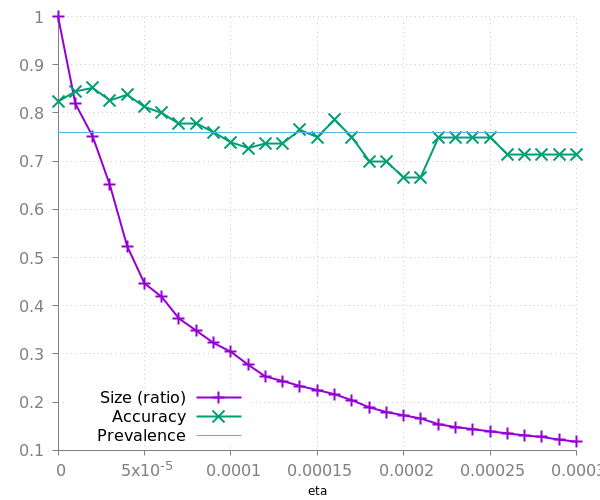
\includegraphics[scale=0.3]{img/meta_adult.png}
\hfill
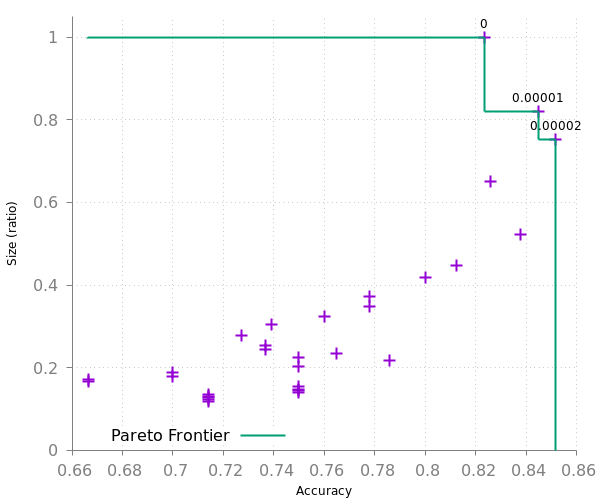
\includegraphics[scale=0.3]{img/meta_pareto_adult.png}
\caption{Influence of $\eta$ on \texttt{adult} dataset.}
\label{fig:meta_adult}
\end{figure}
More work is required to fully study the influence of the hyperparameters $(\eta_{-1}, \eta_1, \bar \eta_{-1}, \bar \eta_1)$ and how to select $l_{-1}$ and $l_1$. We believe it is the key to improve the overall performance, and it is possible to derivate the best values from the training set. Also, a comparison with binary classification methods that provide a prediction confidence metric is necessary.
\begin{figure}[!h]\centering
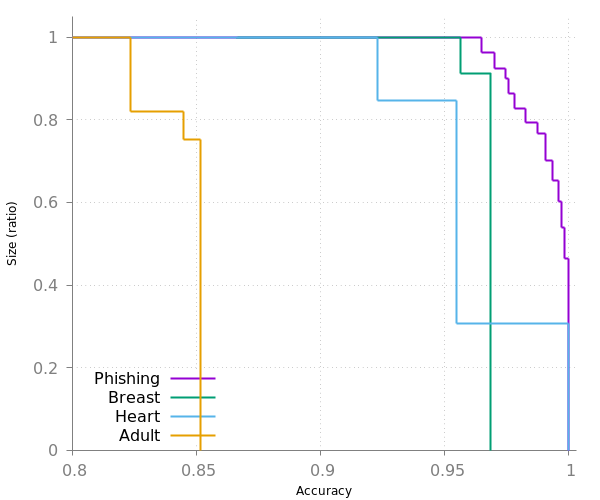
\includegraphics[scale=0.3]{img/meta_pareto_all_front.png}
\caption{Pareto Frontiers comparison.}
\label{fig:meta_all}
\end{figure}

%\newpage
\section{Conclusion}
\label{sec:conclusion}

This paper presented \HCBR, a method for binary classification in unstructured space using a hypergraph representation of information and building a convex combination out of the induced partition to determine the support for each class. The general framework introduced by \eqref{eqn:model} is instantiated in Section \ref{sec:model_selection} and \ref{sec:decision_training} where the support is determined using all the interactions between the hyperedges. Beyond this specific implementation, one can imagine different model selection methods to be used, e.g. using some assumptions on the data.

However, being totally agnostic on the data representation is convenient compared to many methods such as SVM. It allows combining information from multiple sources by simply {\it stacking} the information. It does not require transforming the data to fit the algorithm, often by designing specific ad-hoc metrics.

\HCBR~ has been tested on 7 well-known datasets and demonstrated similar accuracies when compared to the best results from the literature. Additionally, we performed a comparison with 9 alternative methods to find out \HCBR~ along with Neural Network outperform in average with a constant good result. This result is important w.r.t. to the capacity to \HCBR~ to be easily used and deployed in practice. We showed that the model is properly calibrated i.e. the support measure can be seen as a confidence measure on the prediction. 
We empirically validated the exponential worst-case complexity. Finally, we studied the properties and limitations of the model space. The learning curves showed that the model does not overfit on any dataset, has a small variance but tend to have a large bias. To determine if the problem comes from the model space complexity or an inefficient model selection procedure, we used a genetic algorithm to optimize an auxiliary function and have shown that the model selection procedure provides one of the best possible performance within the model space. Hence, further work will focus on extending the model space.

This proof of concept raises many questions and offer many improvement axes. First of all, it seems relatively easy to extend the method to several classes but it needs an additional empirical validation. As most of the computational effort is on calculating the class support, adding more classes will linearly increase the computation time and thus, working on a faster algorithm or an approximation of the main measure should be investigated. The solution may come from exploring the feature selection capacity of \HCBR. Indeed, by the hypergraph construction, it may be possible to remove from the partition some elements that do not participate enough (e.g. not being in enough cases at the same time), reducing the computation time.
Additionally, we plan to investigate how to generate an explanation about each prediction and one about the decision function $J$ itself, using not only the convex combination and the strength of the partition elements, but also the link between cases in a similar way a lawyer may use past cases to make analogies or counter-examples. We also work on an online version of \HCBR~ where the hypergraph is constructed case after case, including forgetting some old past cases (which would allow handling non-stationary environment). It seems also possible not only to add new examples dynamically, but also some vertices (i.e. adding some pertinent information to some cases) without generating the whole model from scratch. 

Empirically, further experiments should focus on more unstructured datasets (for instance for text classification). As stated previously, strategies for hyperparameter tunning are also a priority.
Last but not least, we would like to answer some questions: can we provide some quality bounds depending on the initial hypergraph and thus the dataset? How to handle continuous values without discretization?

\section*{Acknowledgment}

The author warmly thanks Dr. Jean-Fran\c{c}ois Puget, IBM Analytics, for their useful suggestions and advice to improve this paper.



\section*{References}

\bibliography{paper}

\end{document}